\section{Задание 1}

Выставлена дата начала проекта.

\begin{figure}[ht!]
	
\includegraphics[width=0.75\linewidth]{assets/images/1-start.png}
	\label{fig:r2}
	\caption{Начало проекта}
\end{figure}
\FloatBarrier

Установлена длительность работы в днях, объем работ в часах, а тип задач по умолчанию --- с фиксированными трудозатратами.

\begin{figure}[ht!]
	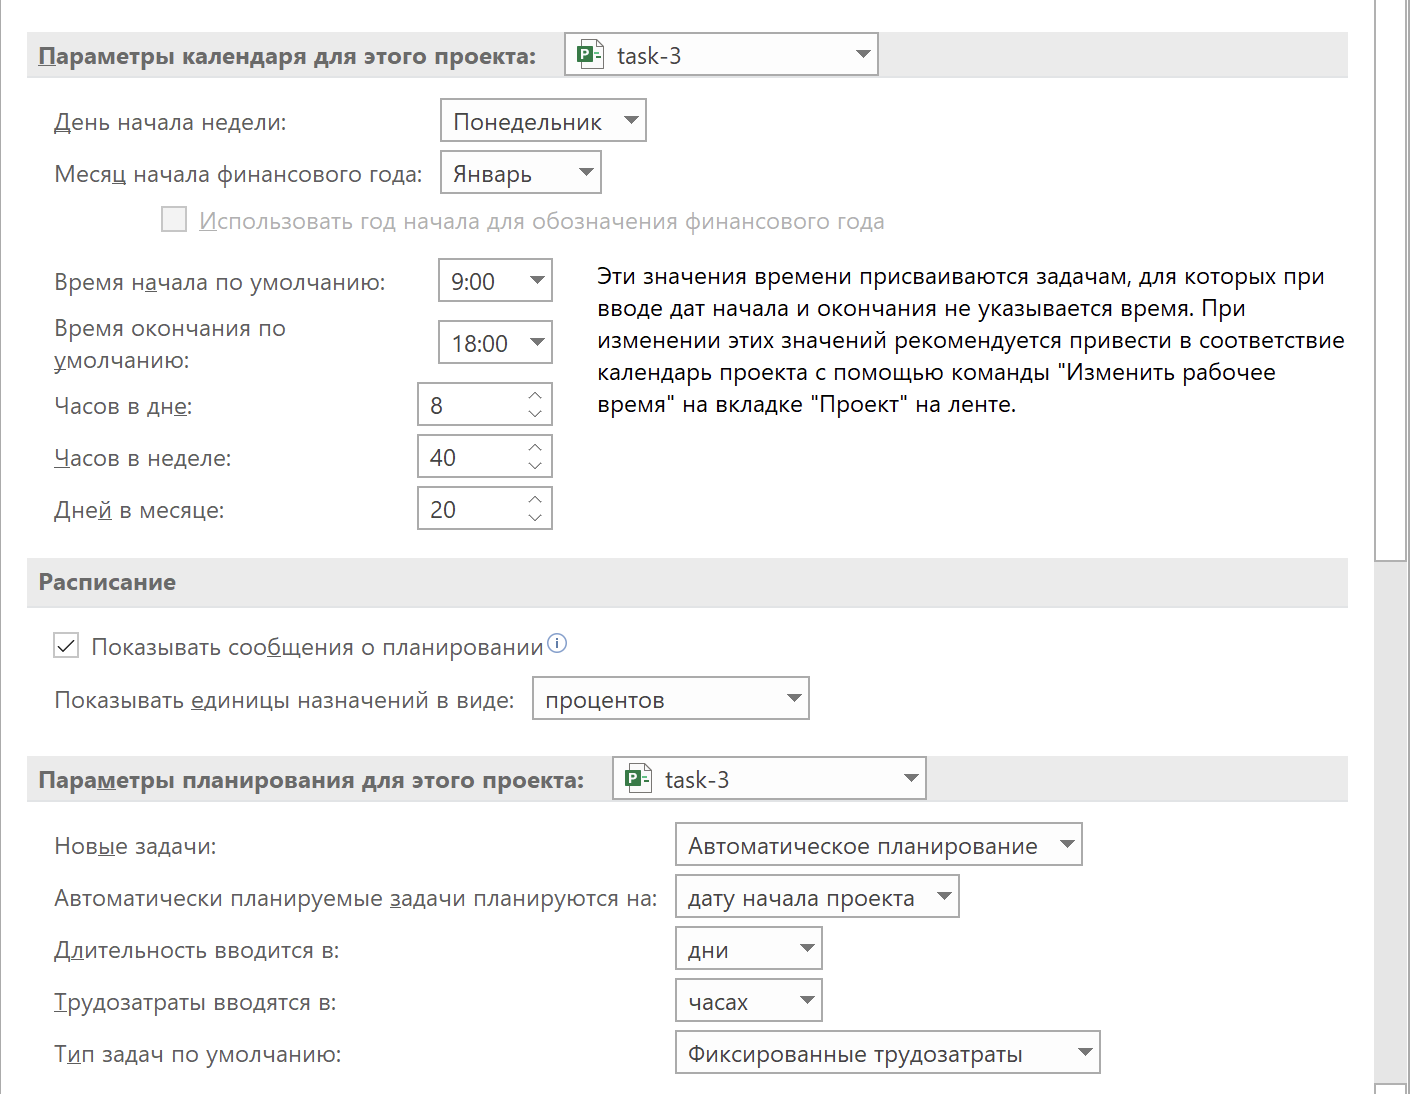
\includegraphics[width=0.75\linewidth]{assets/images/1-long.png}
	\label{fig:r2}
	\caption{Длительность}
\end{figure}
\FloatBarrier

Учтены праздничные дни, попадающие на период реализации проекта.

\begin{figure}[ht!]
	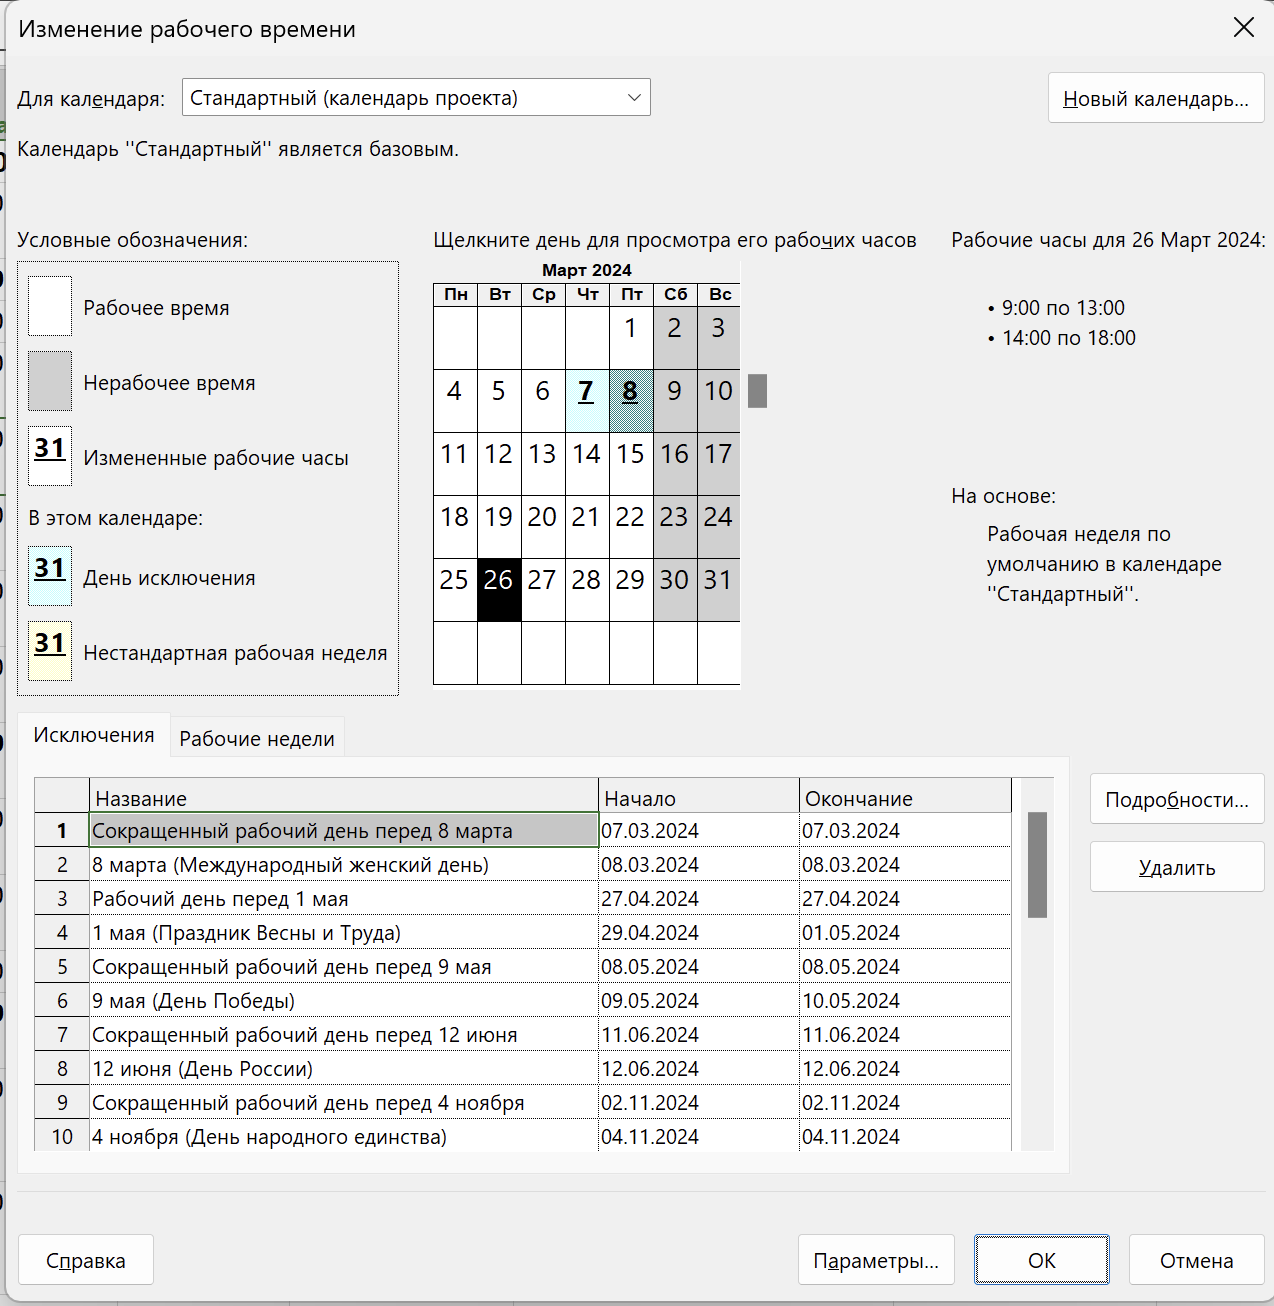
\includegraphics[width=0.75\linewidth]{assets/images/1-calendar.png}
	\label{fig:r2}
	\caption{Календарь}
\end{figure}
\FloatBarrier

\section{Задание 2}

Задачи были заданы в соотвествии с вариантом.

\begin{figure}[ht!]
	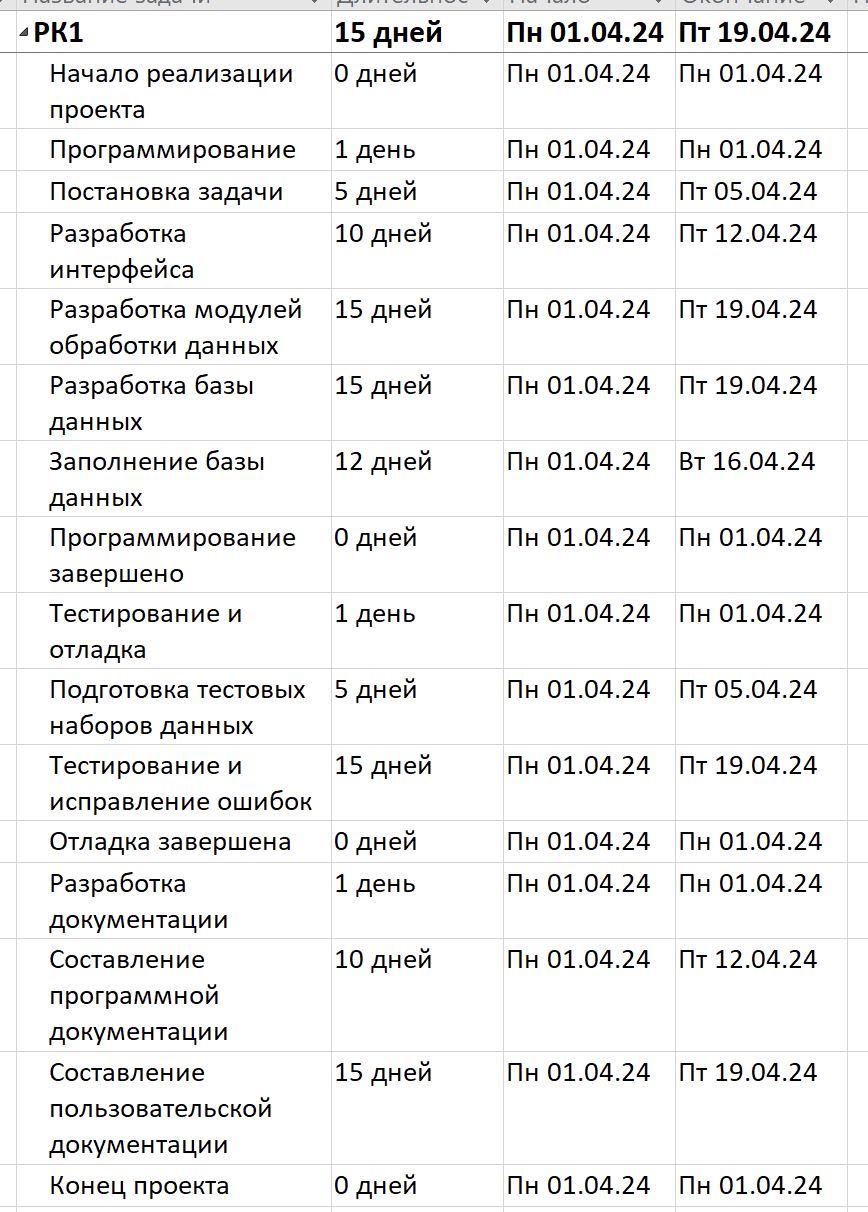
\includegraphics[width=0.75\linewidth]{assets/images/2-tasks.png}
	\label{fig:r2}
	\caption{Задачи}
\end{figure}
\FloatBarrier


\section{Задание 3}

Задачи структурированы.

\begin{figure}[ht!]
	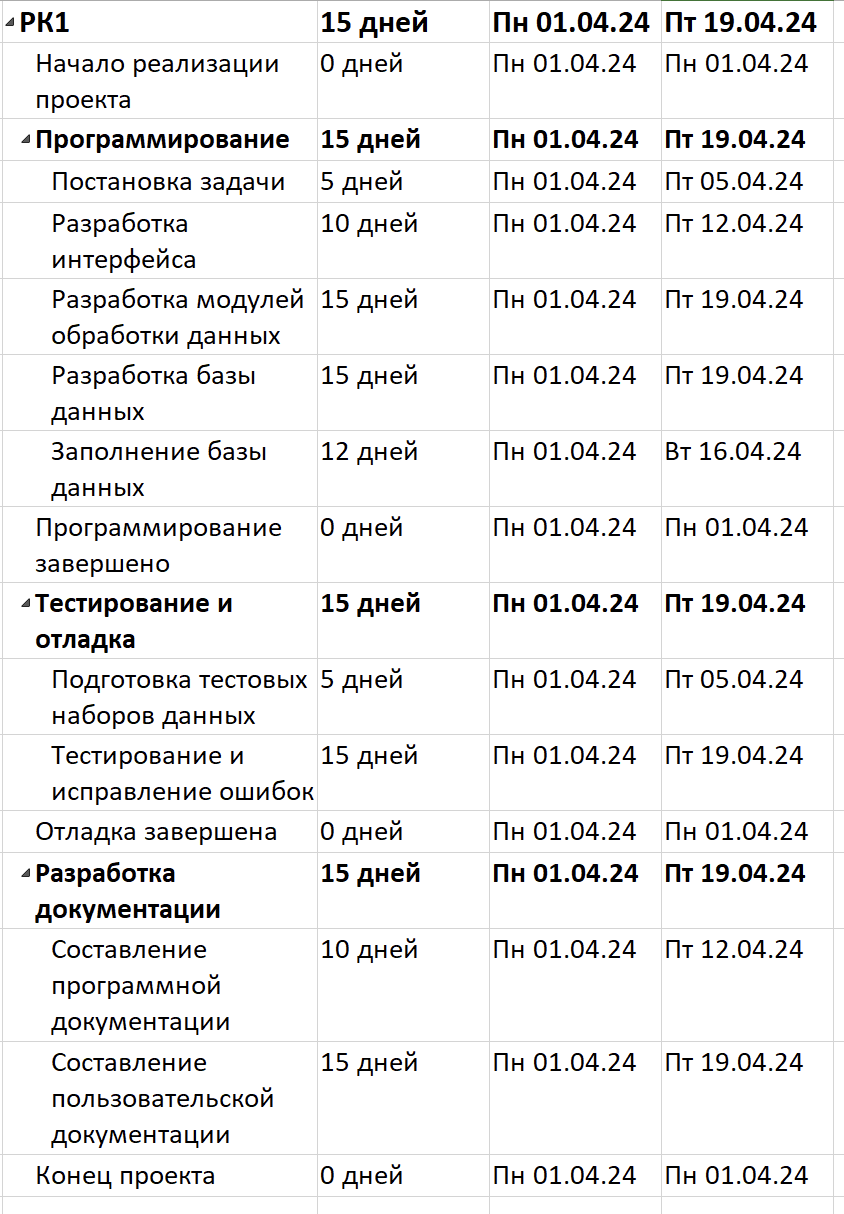
\includegraphics[width=0.75\linewidth]{assets/images/3-tasks.png}
	\label{fig:r2}
	\caption{Задачи}
\end{figure}
\FloatBarrier

\section{Задание 4}

Задачи связаны.

\begin{figure}[ht!]
	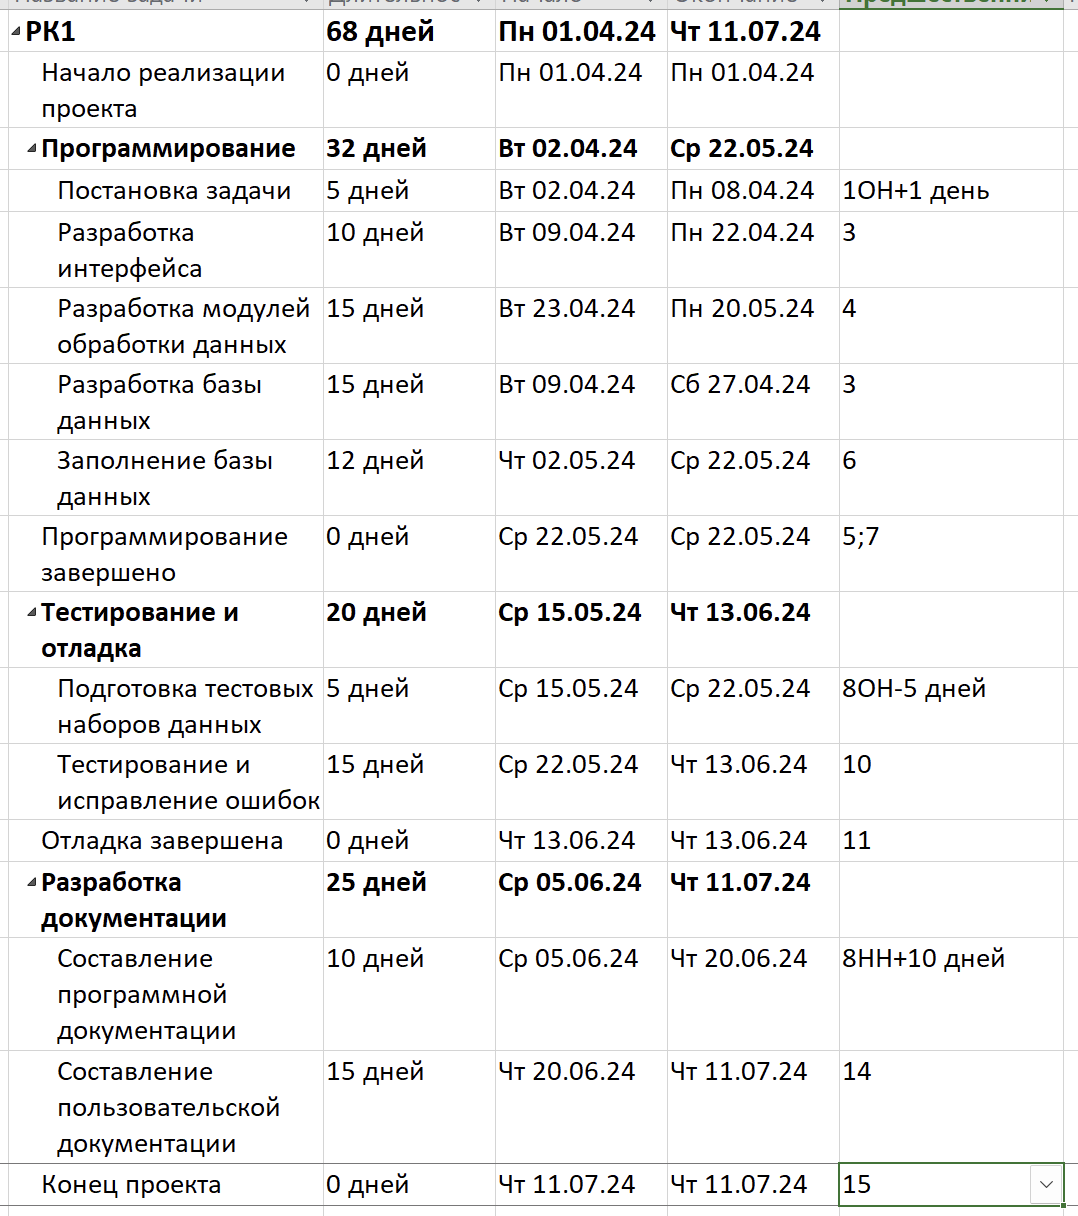
\includegraphics[width=0.75\linewidth]{assets/images/4-task.png}
	\label{fig:r2}
	\caption{Задачи}
\end{figure}
\FloatBarrier


\section{Задание 5}

Назанчены ресурсы в соотвествии с заданием.

\begin{figure}[ht!]
	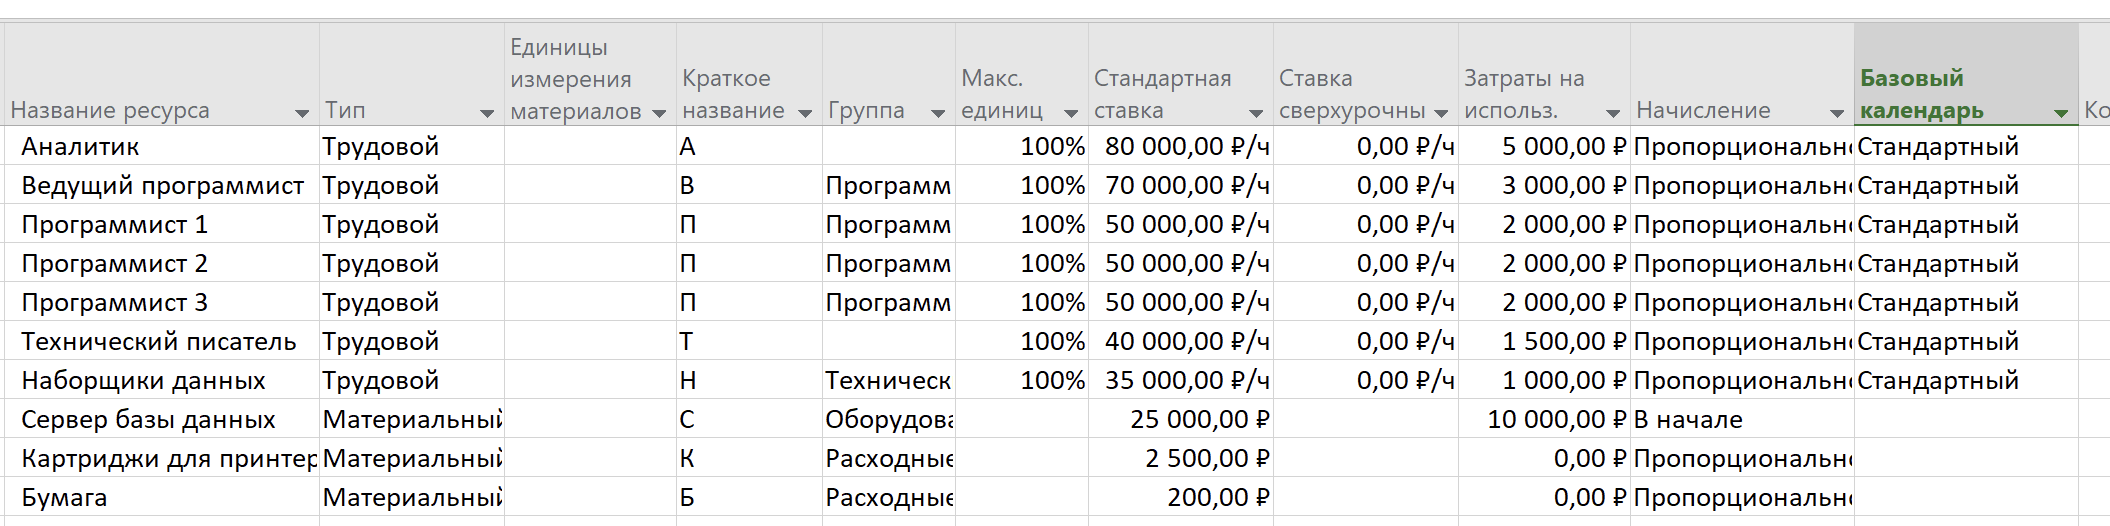
\includegraphics[width=0.75\linewidth]{assets/images/5-task.png}
	\label{fig:r2}
	\caption{Ресурсы}
\end{figure}
\FloatBarrier

\section{Задание 6}

Назаначены ресурсы в сооствествии с заданием, возникли перезгрузки.

\begin{figure}[ht!]
	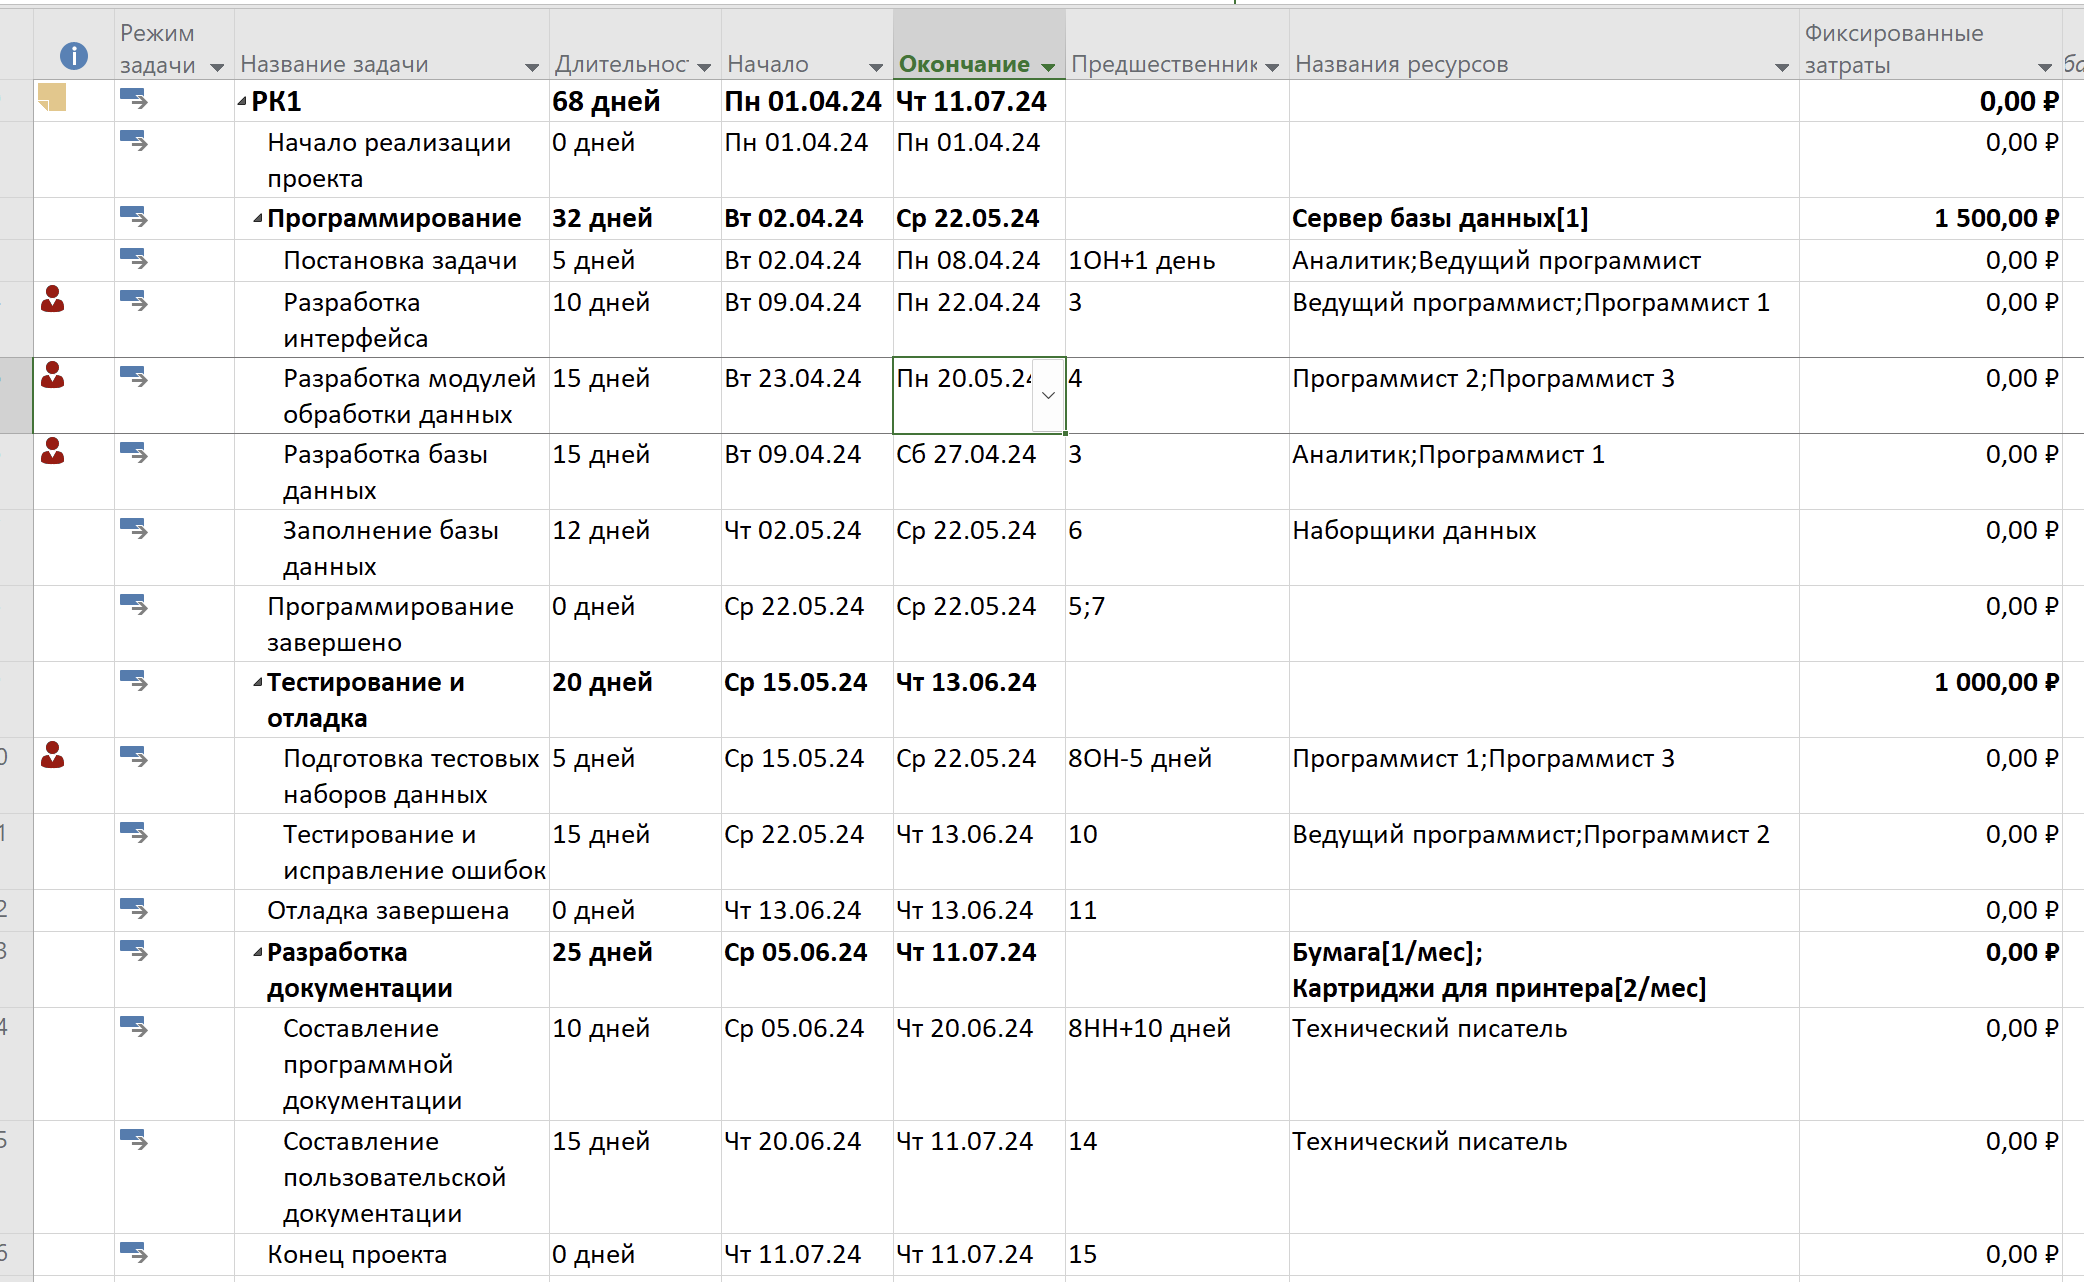
\includegraphics[width=0.75\linewidth]{assets/images/6-tasks.png}
	\label{fig:r2}
	\caption{Ресурсы}
\end{figure}
\FloatBarrier

\section{Задание 7}

Перегрузки устранены с помощью автоматического выравнивания.

\begin{figure}[ht!]
	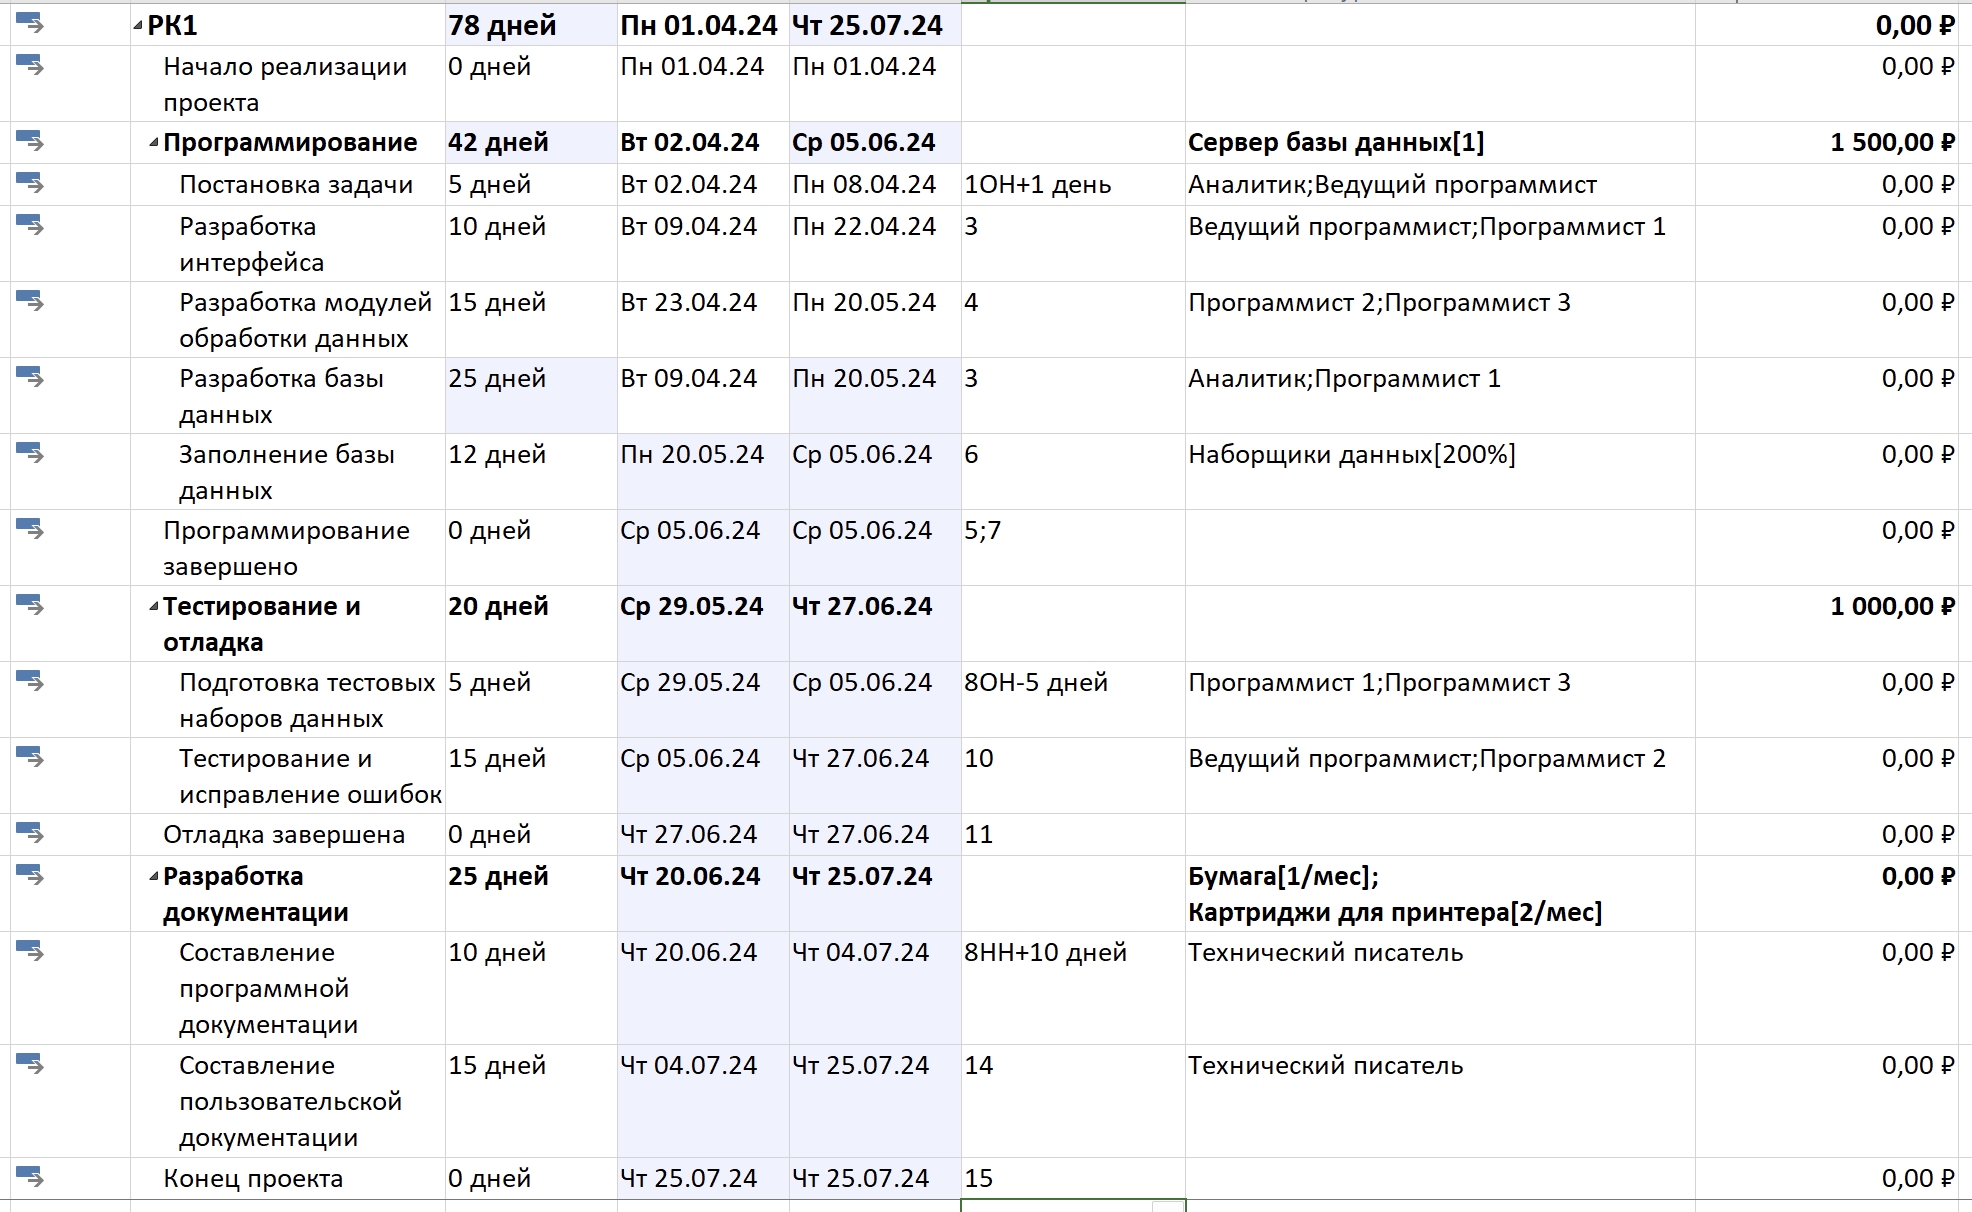
\includegraphics[width=0.75\linewidth]{assets/images/7-tasks.png}
	\label{fig:r2}
	\caption{Ресурсы}
\end{figure}
\FloatBarrier

\begin{figure}[ht!]
	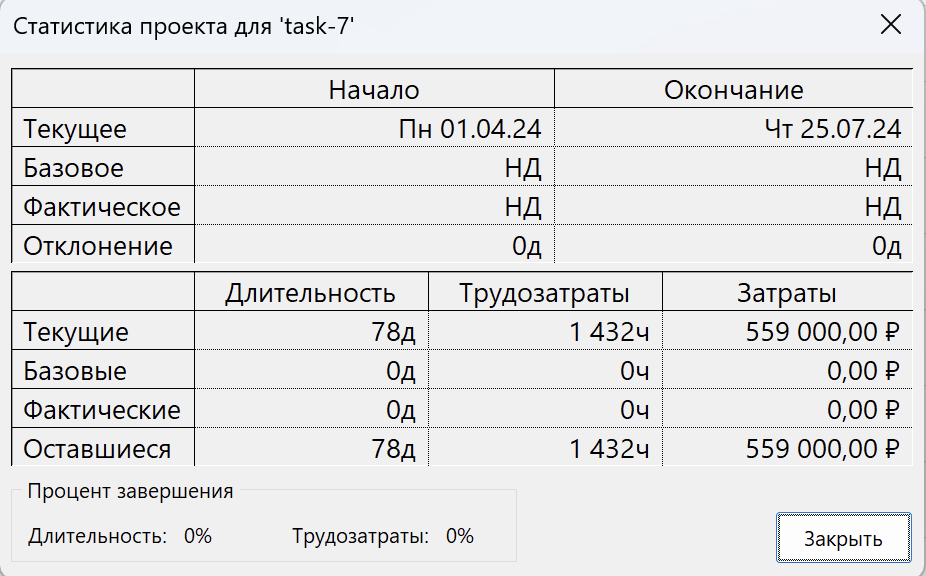
\includegraphics[width=0.75\linewidth]{assets/images/7-zatrat.png}
	\label{fig:r2}
	\caption{Ресурсы}
\end{figure}
\FloatBarrier


\section{Задание 8}

Включена профелактика оборудования

\begin{figure}[ht!]
	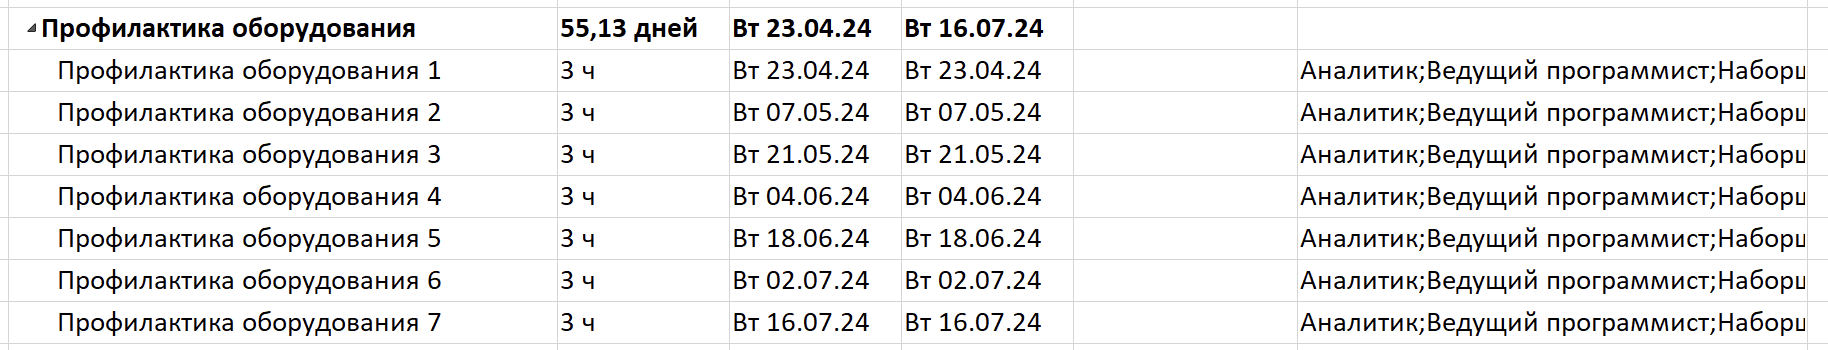
\includegraphics[width=0.75\linewidth]{assets/images/8.1-check.png}
	\label{fig:r2}
	\caption{Профелактика оборудования}
\end{figure}
\FloatBarrier

Назаначен материальный ресурс для аутсорсной компании.


\begin{figure}[ht!]
	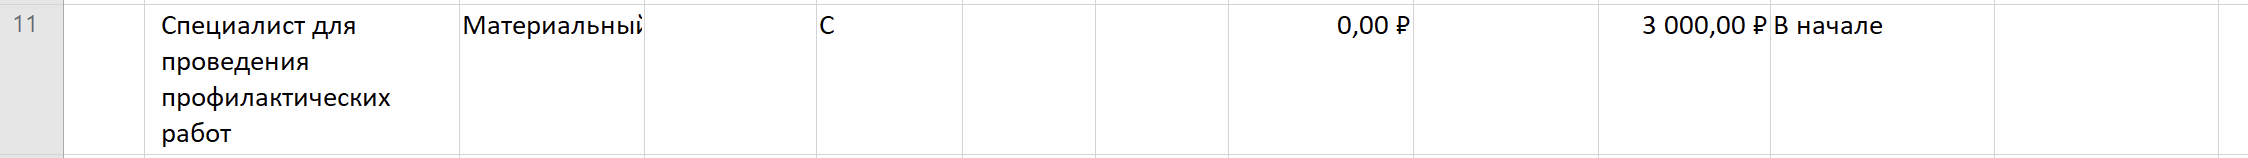
\includegraphics[width=0.75\linewidth]{assets/images/8.2-outsource.png}
	\label{fig:r2}
	\caption{Профелактика оборудования}
\end{figure}
\FloatBarrier

Чтобы задачу нельзя было выполнять параллельно, была назанчены все ресурсы на эту задачу с нулевым зарплатным проектом.

\begin{figure}[ht!]
	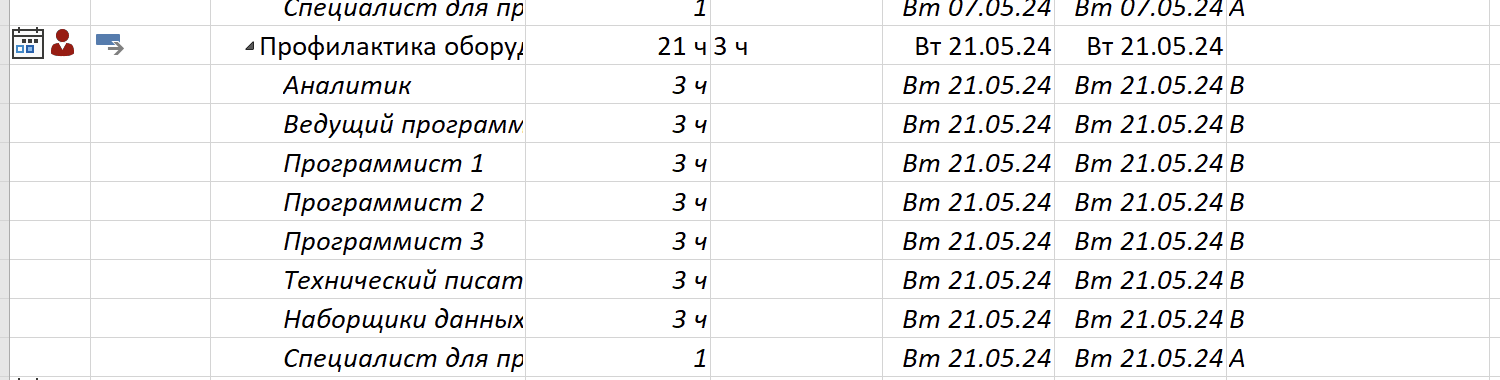
\includegraphics[width=0.75\linewidth]{assets/images/8.3-conflicts.png}
	\label{fig:r2}
	\caption{Профелактика оборудования}
\end{figure}
\FloatBarrier

При выставлении данной задачи возникли конфликты, которые были решены автоматическим выравниванием.
Проект стал заканчиваться 29.04.2024.

\begin{figure}[ht!]
	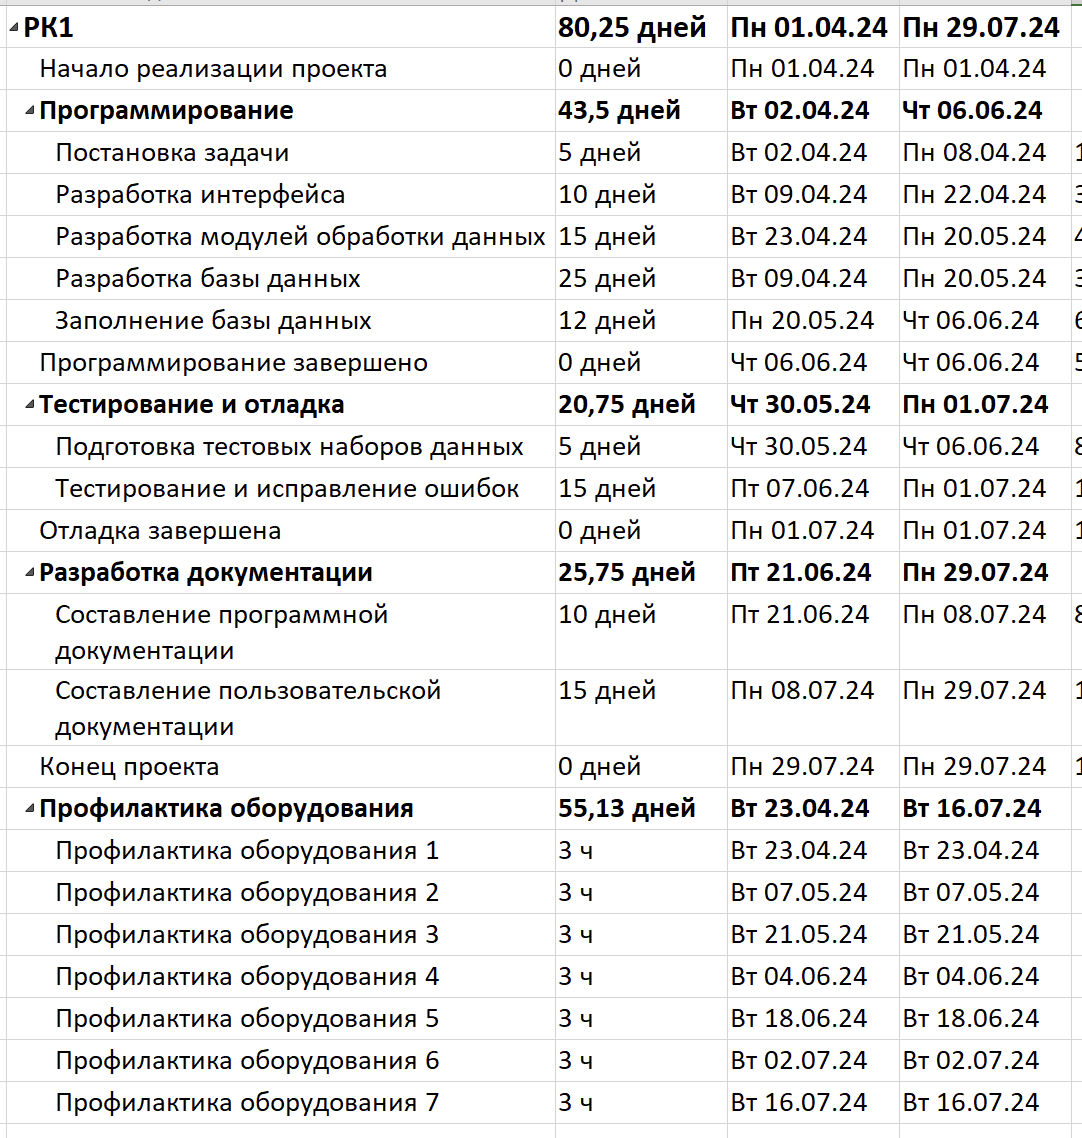
\includegraphics[width=0.75\linewidth]{assets/images/8.4-conf.png}
	\label{fig:r2}
	\caption{Профелактика оборудования}
\end{figure}
\FloatBarrier

На данный момент стоимость проекта составляет:

\begin{figure}[ht!]
	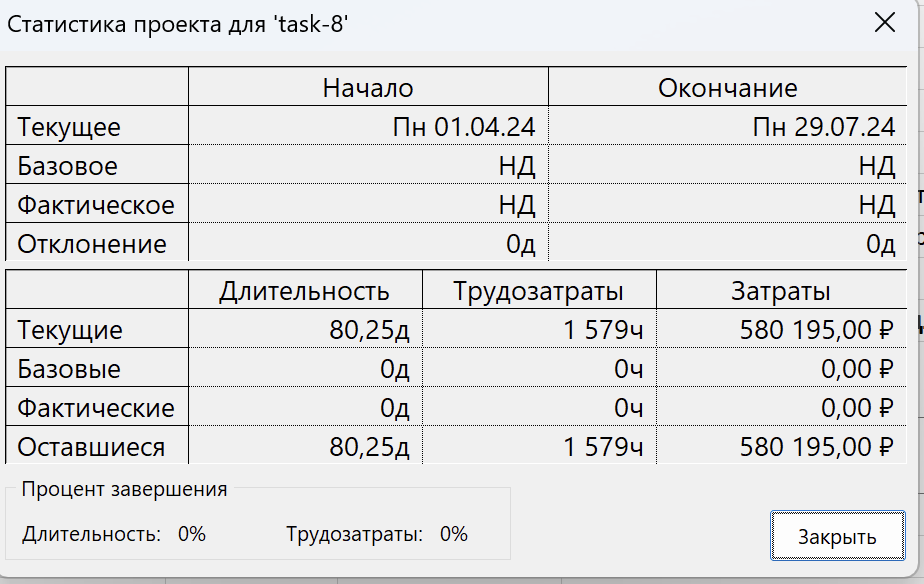
\includegraphics[width=0.75\linewidth]{assets/images/8.5-zatrats.png}
	\label{fig:r2}
	\caption{Профелактика оборудования}
\end{figure}
\FloatBarrier

\section{Задание 9}

Критический путь выглядит так:

\begin{figure}[ht!]
	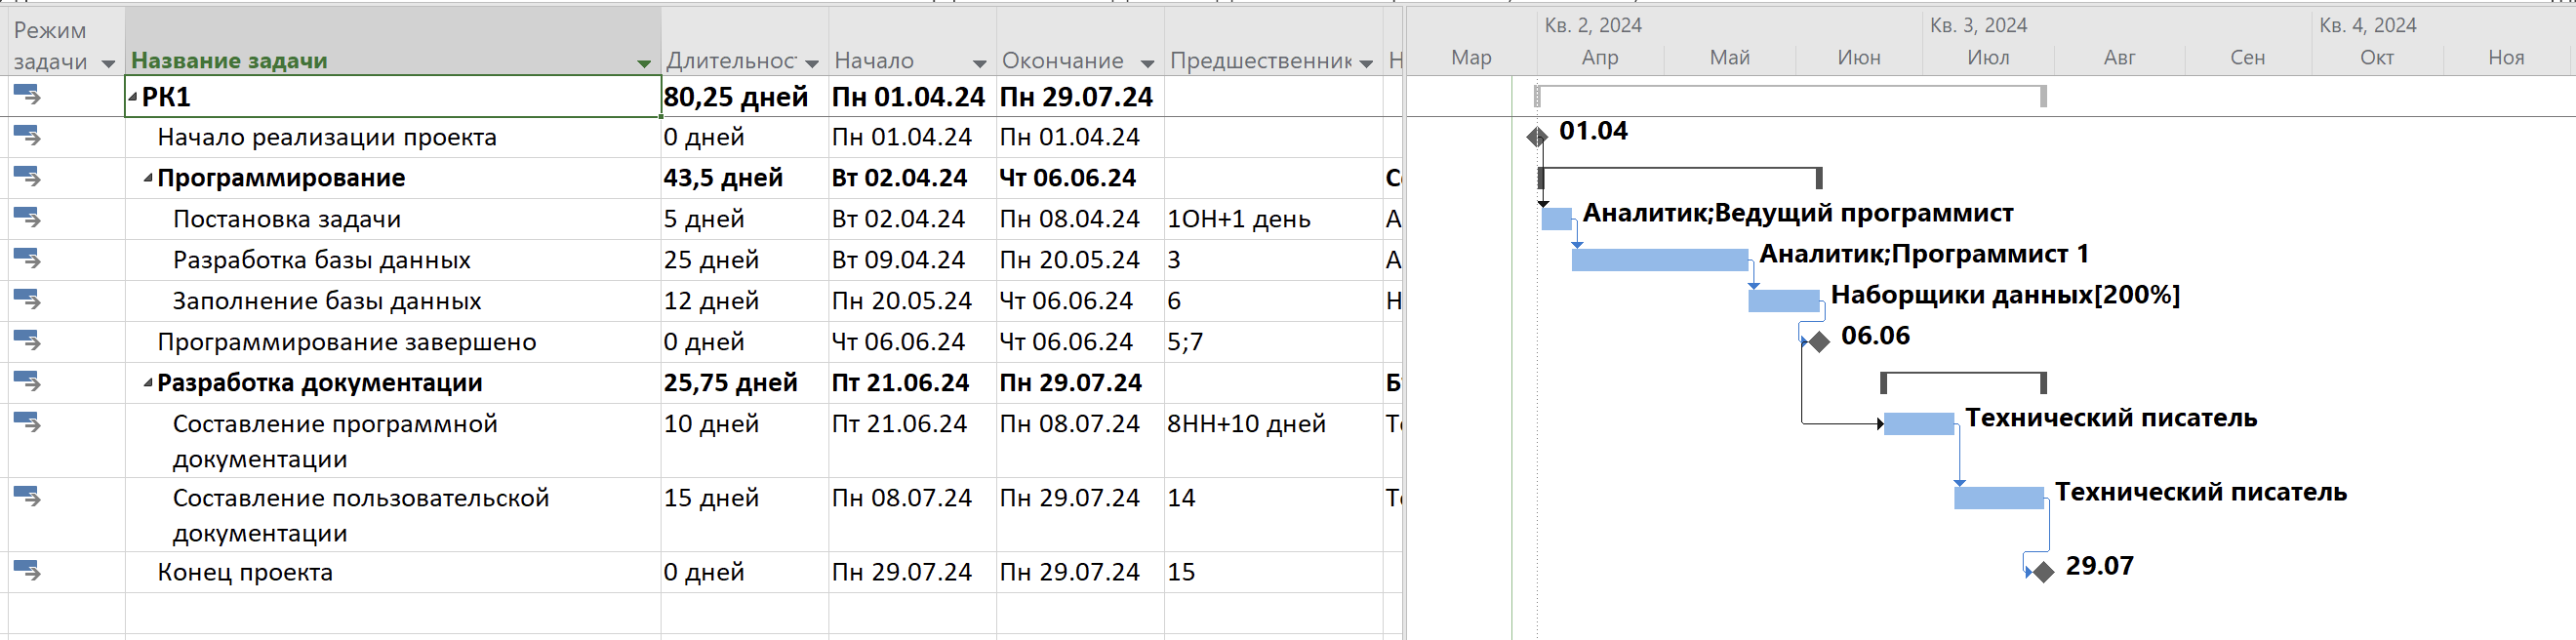
\includegraphics[width=0.75\linewidth]{assets/images/9.1-crit.png}
	\label{fig:r2}
	\caption{Оптимизация}
\end{figure}
\FloatBarrier

На задачу разработка базы данных было назанчено больше программистов.

\begin{figure}[ht!]
	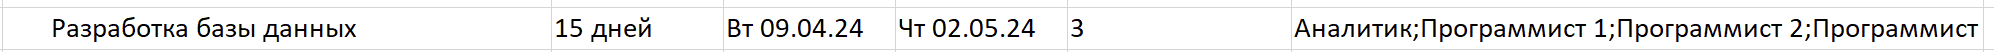
\includegraphics[width=0.75\linewidth]{assets/images/9.2-optimiz.png}
	\label{fig:r2}
	\caption{Оптимизация}
\end{figure}
\FloatBarrier

Срок сдвинулся на 15.07. То есть на 13 дней (с 29.07)

\begin{figure}[ht!]
	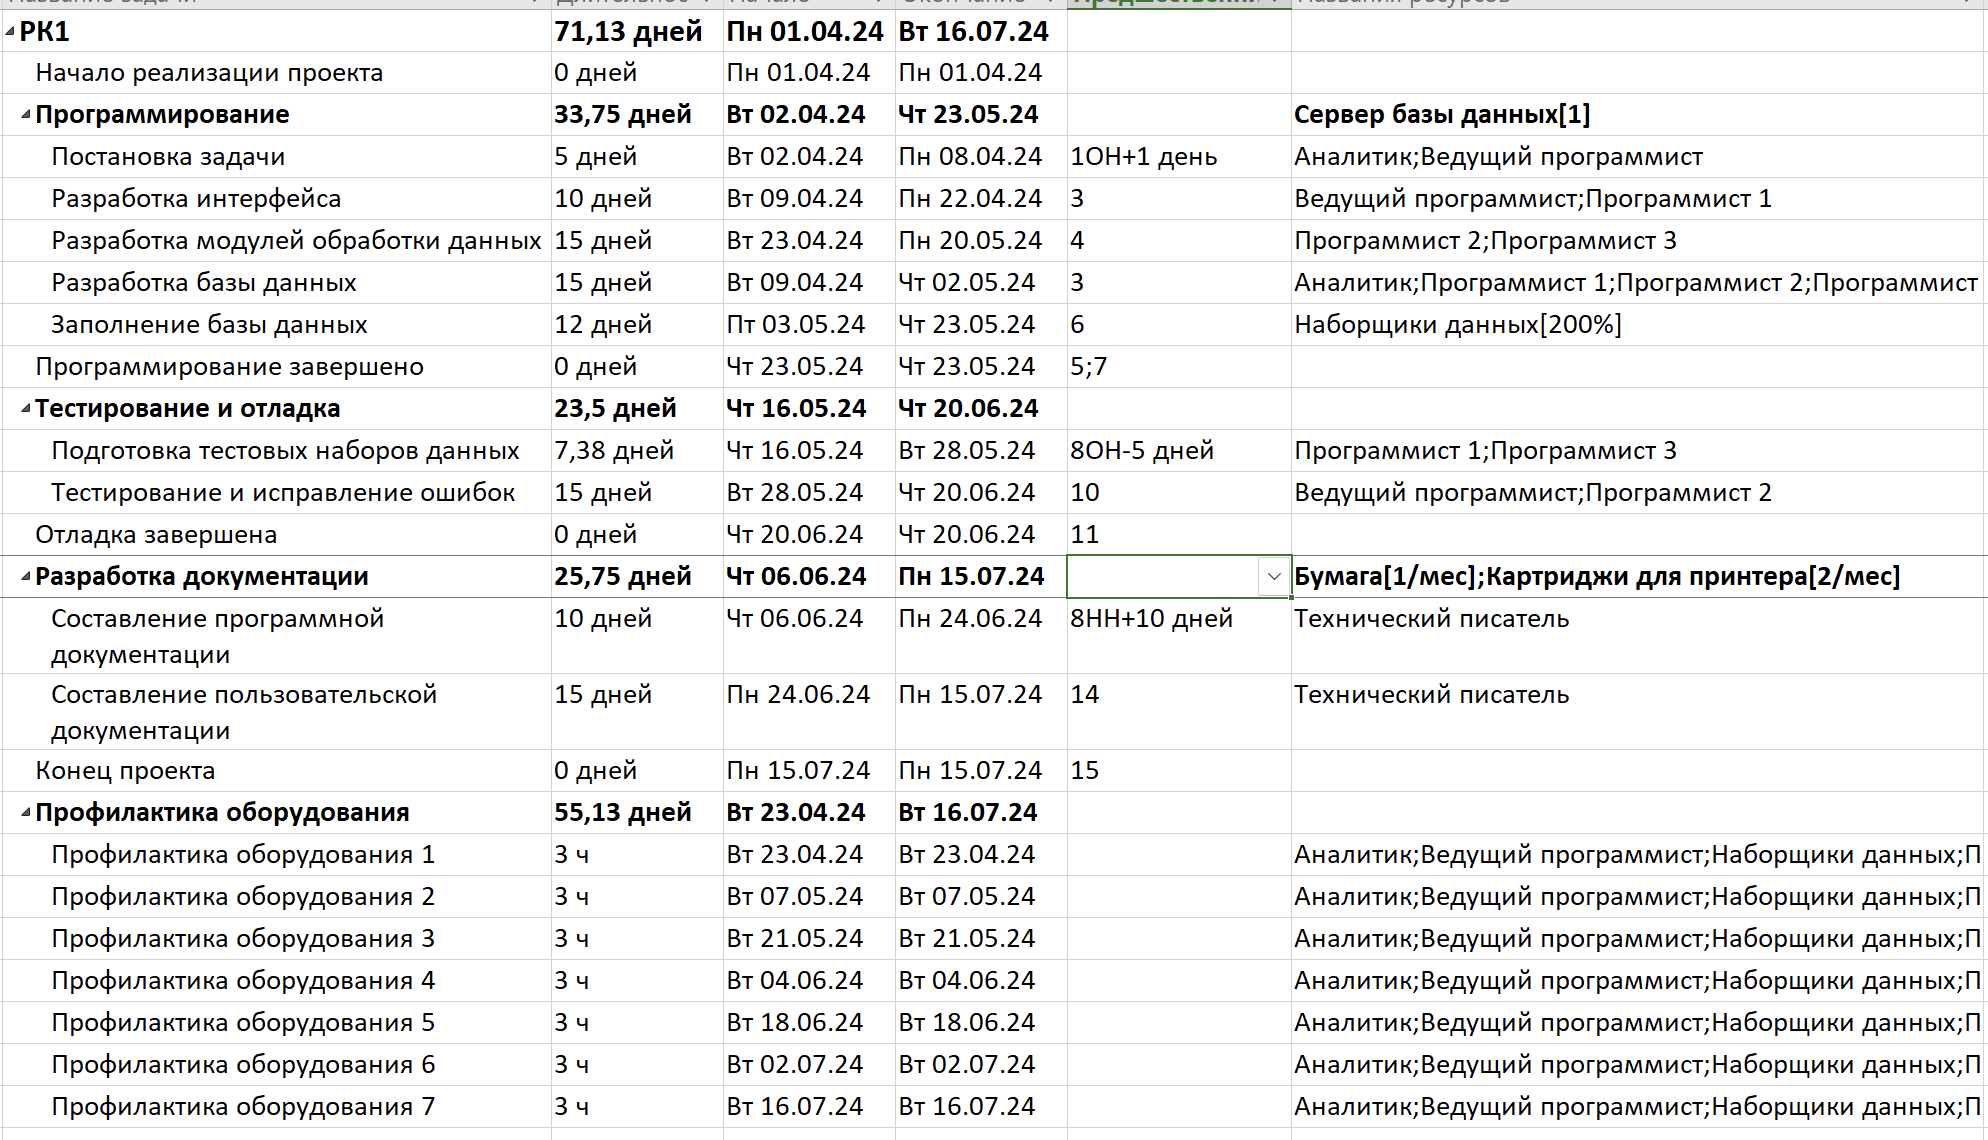
\includegraphics[width=0.75\linewidth]{assets/images/9.3-res.png}
	\label{fig:r2}
	\caption{Оптимизация}
\end{figure}
\FloatBarrier

Затарты на проект сократились до 570132.50.

\begin{figure}[ht!]
	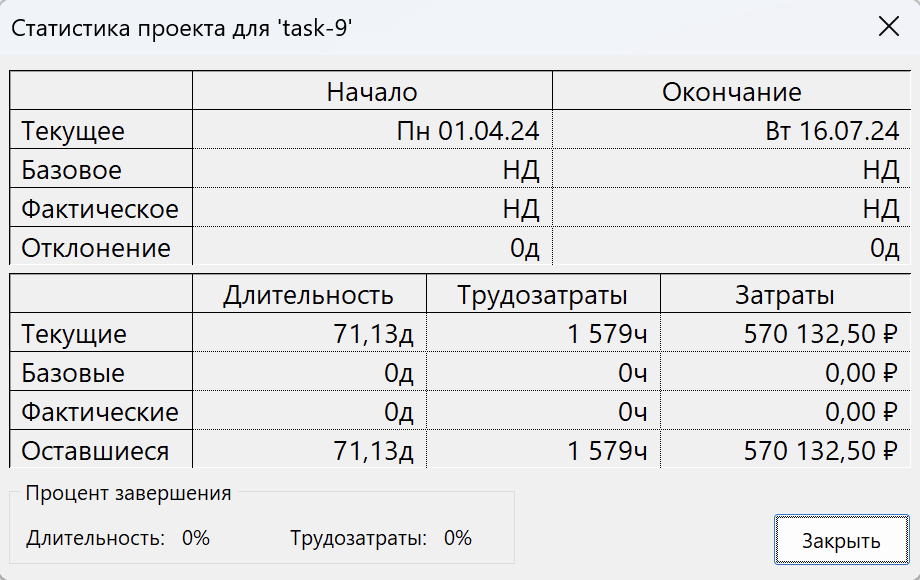
\includegraphics[width=0.75\linewidth]{assets/images/9.4-zatrat.png}
	\label{fig:r2}
	\caption{Оптимизация}
\end{figure}
\FloatBarrier

\section{Задание 10}

Назначена дата отчета на 21.06.

\begin{figure}[ht!]
	
\includegraphics[width=0.75\linewidth]{assets/images/10.1-othet.png}
	\label{fig:r2}
	\caption{Оптимизация}
\end{figure}
\FloatBarrier

Программист 2 заболел на недели.

\begin{figure}[ht!]
	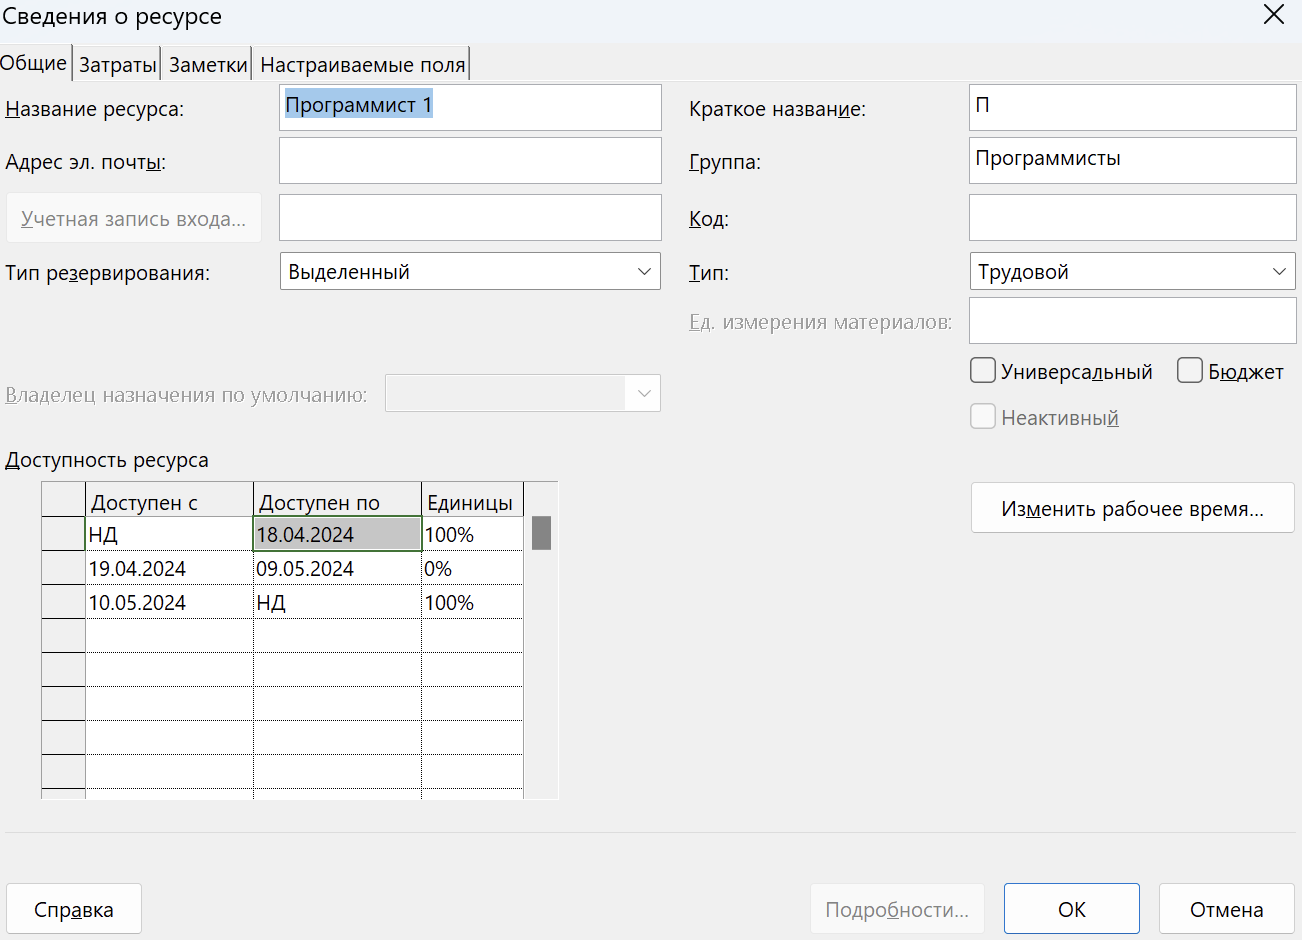
\includegraphics[width=0.75\linewidth]{assets/images/10.2-progdie.png}
	\label{fig:r2}
	\caption{Ухудшаем ситуацию}
\end{figure}
\FloatBarrier

Срок сдвинулся на 5 августа

\begin{figure}[ht!]
	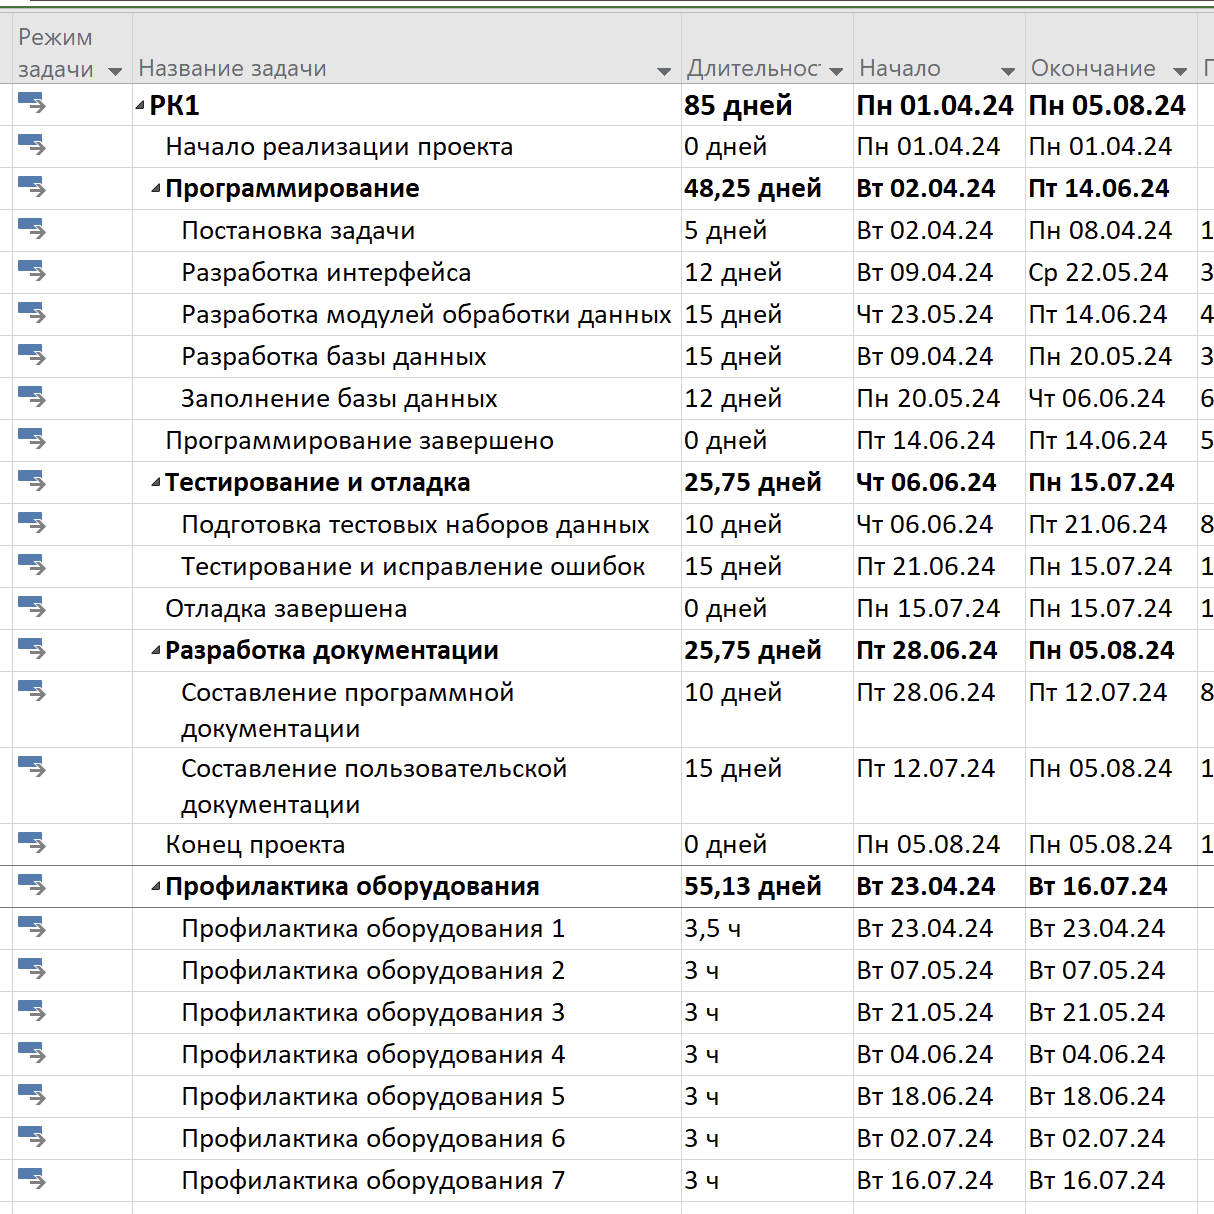
\includegraphics[width=0.75\linewidth]{assets/images/10.2.2-zabolel.png}
	\label{fig:r2}
	\caption{Ухудшаем ситуацию}
\end{figure}
\FloatBarrier

Аналитик захотел больше денег с 3 апреля на 50 процентов

\begin{figure}[ht!]
	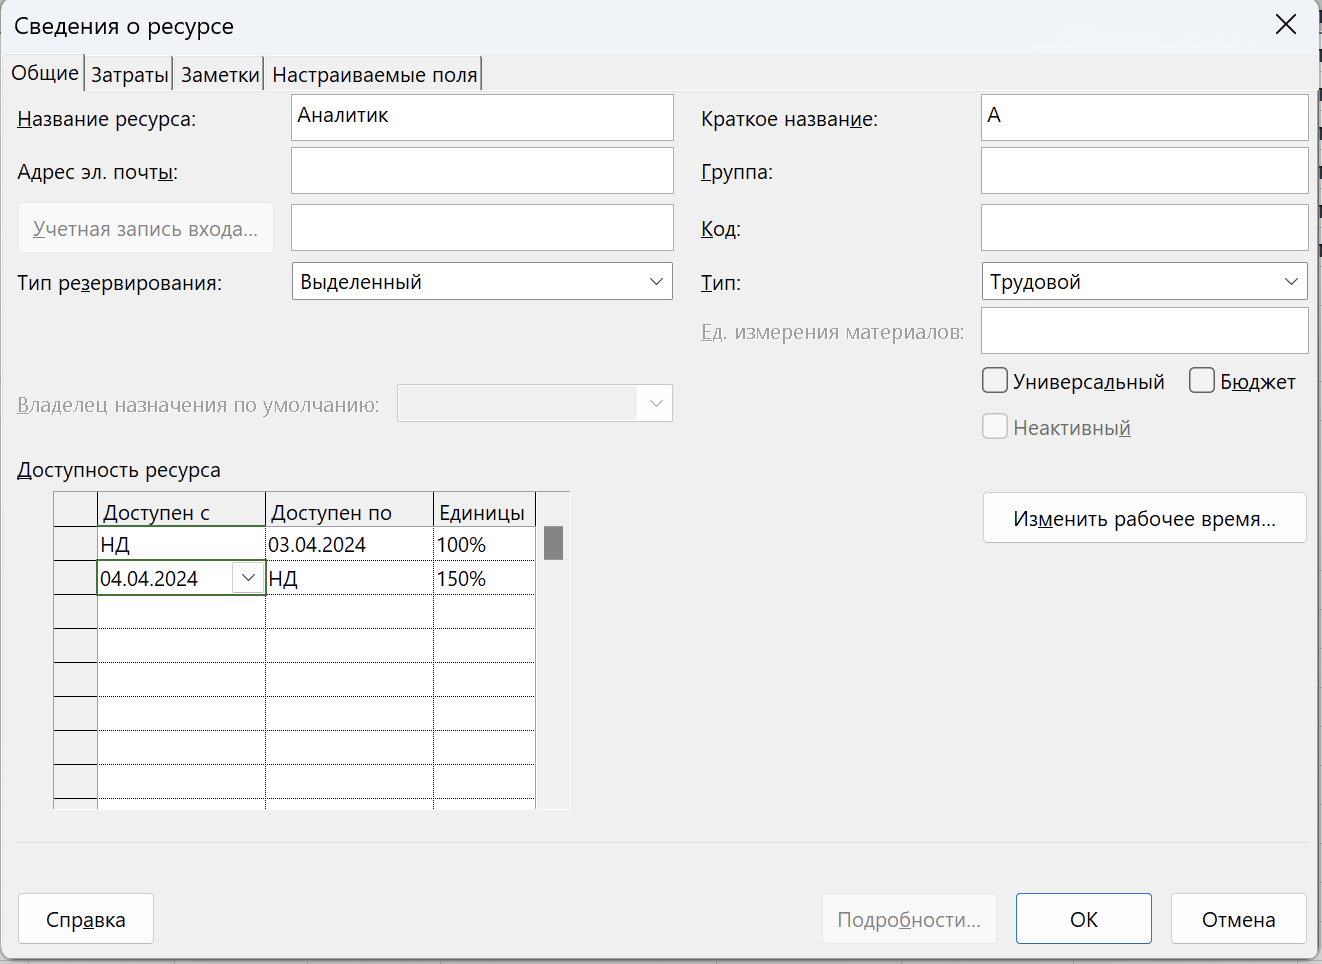
\includegraphics[width=0.75\linewidth]{assets/images/10.3-debil.png}
	\label{fig:r2}
	\caption{Ухудшаем ситуацию}
\end{figure}
\FloatBarrier

Ведущий программист решил поработать на полставки с 11.04 до 09.05.

\begin{figure}[ht!]
	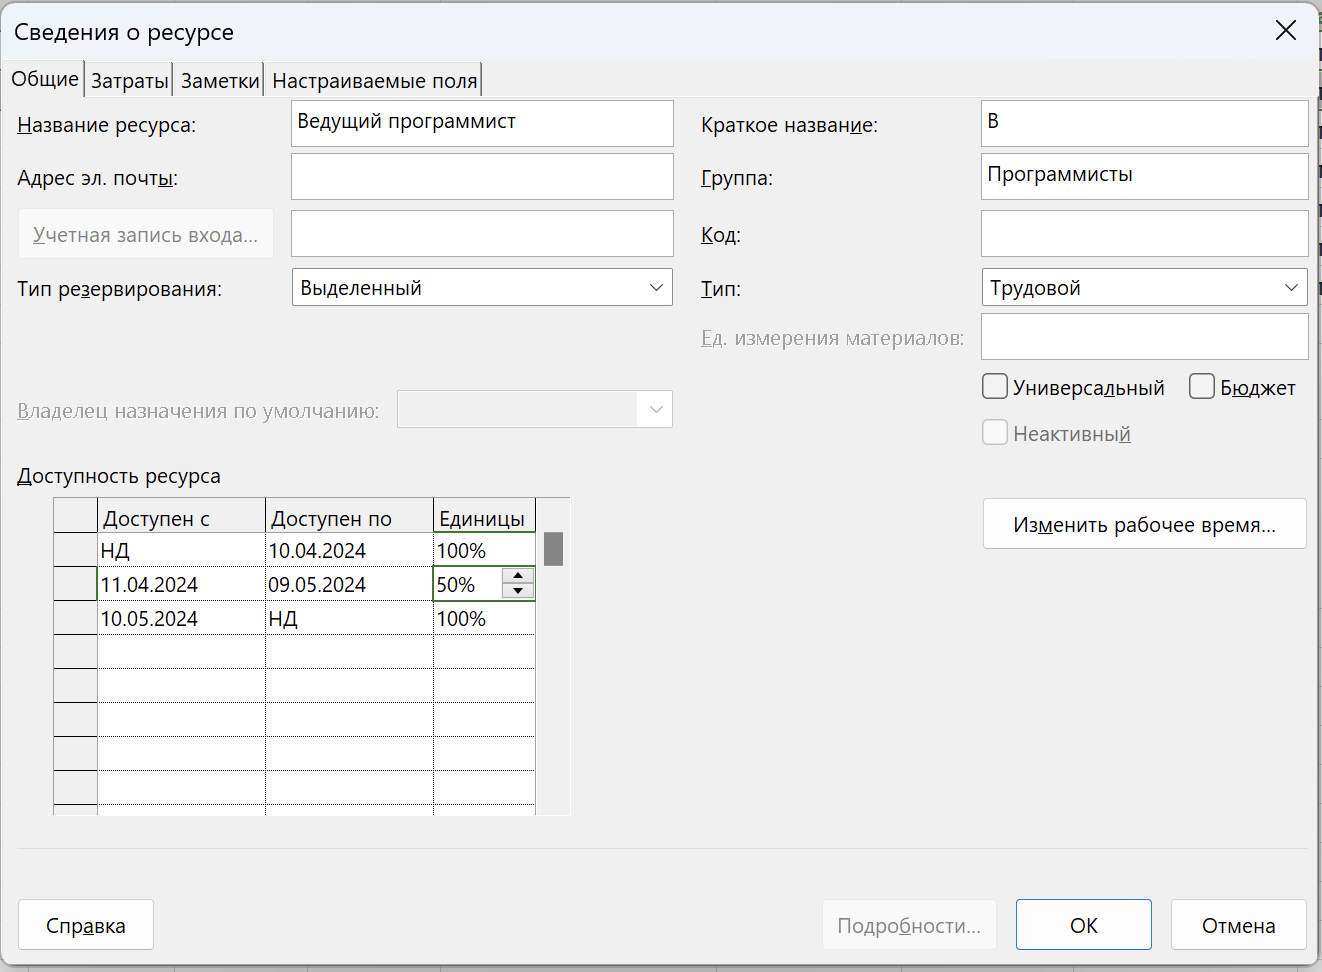
\includegraphics[width=0.75\linewidth]{assets/images/10.4-vedush.png}
	\label{fig:r2}
	\caption{Ухудшаем ситуацию}
\end{figure}
\FloatBarrier

Одна задача стала дольше на полдня.

\begin{figure}[ht!]
	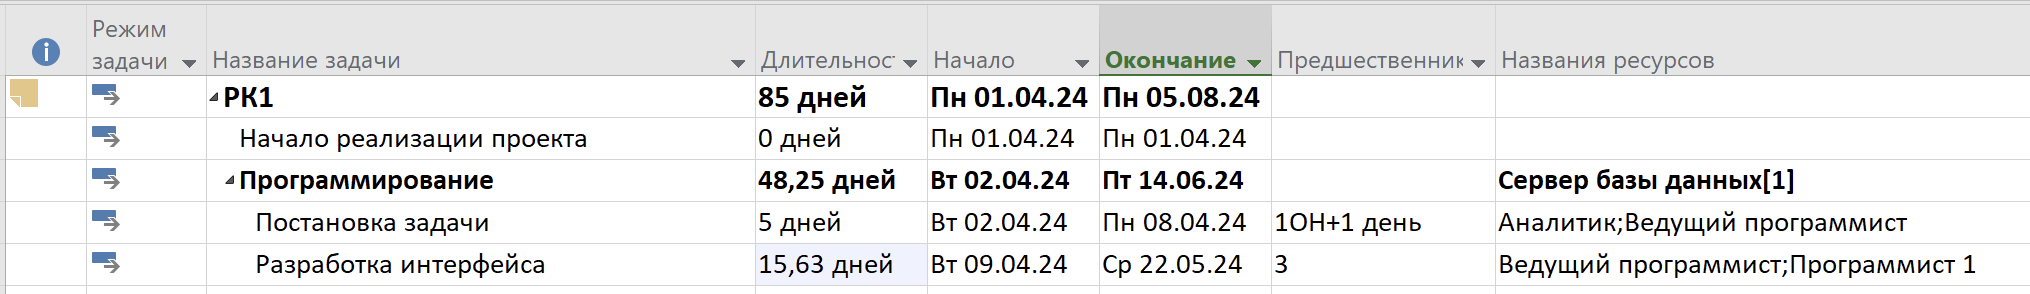
\includegraphics[width=0.75\linewidth]{assets/images/10.4.2-vedush.png}
	\label{fig:r2}
	\caption{Ухудшаем ситуацию}
\end{figure}
\FloatBarrier

Технический писатель заболел в июле.

\begin{figure}[ht!]
	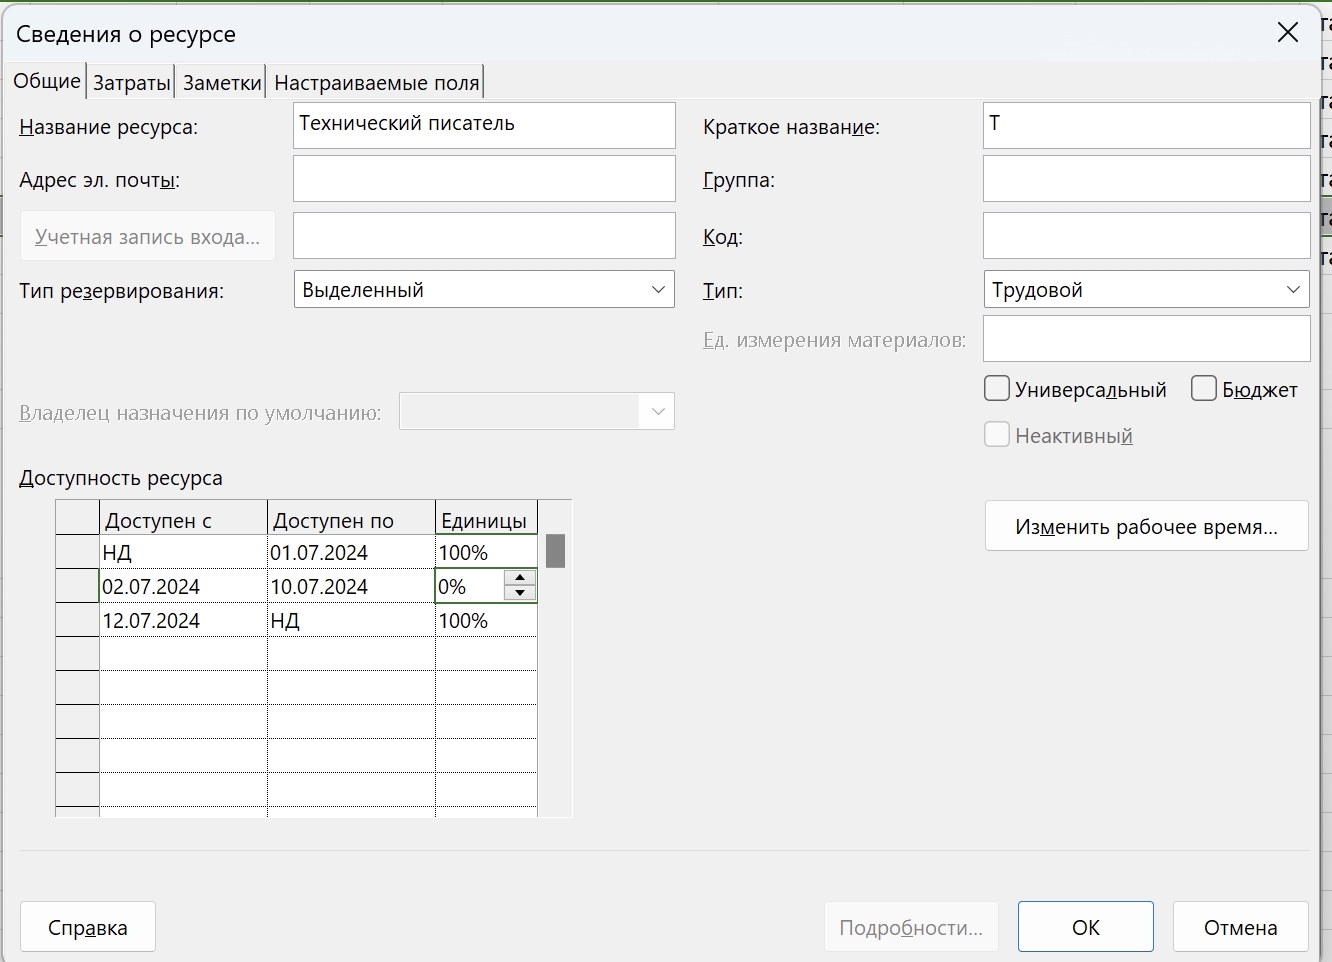
\includegraphics[width=0.75\linewidth]{assets/images/10.5.1-pisaka.png}
	\label{fig:r2}
	\caption{Ухудшаем ситуацию}
\end{figure}
\FloatBarrier

Сроки сдвинулись до 14.08.

\begin{figure}[ht!]
	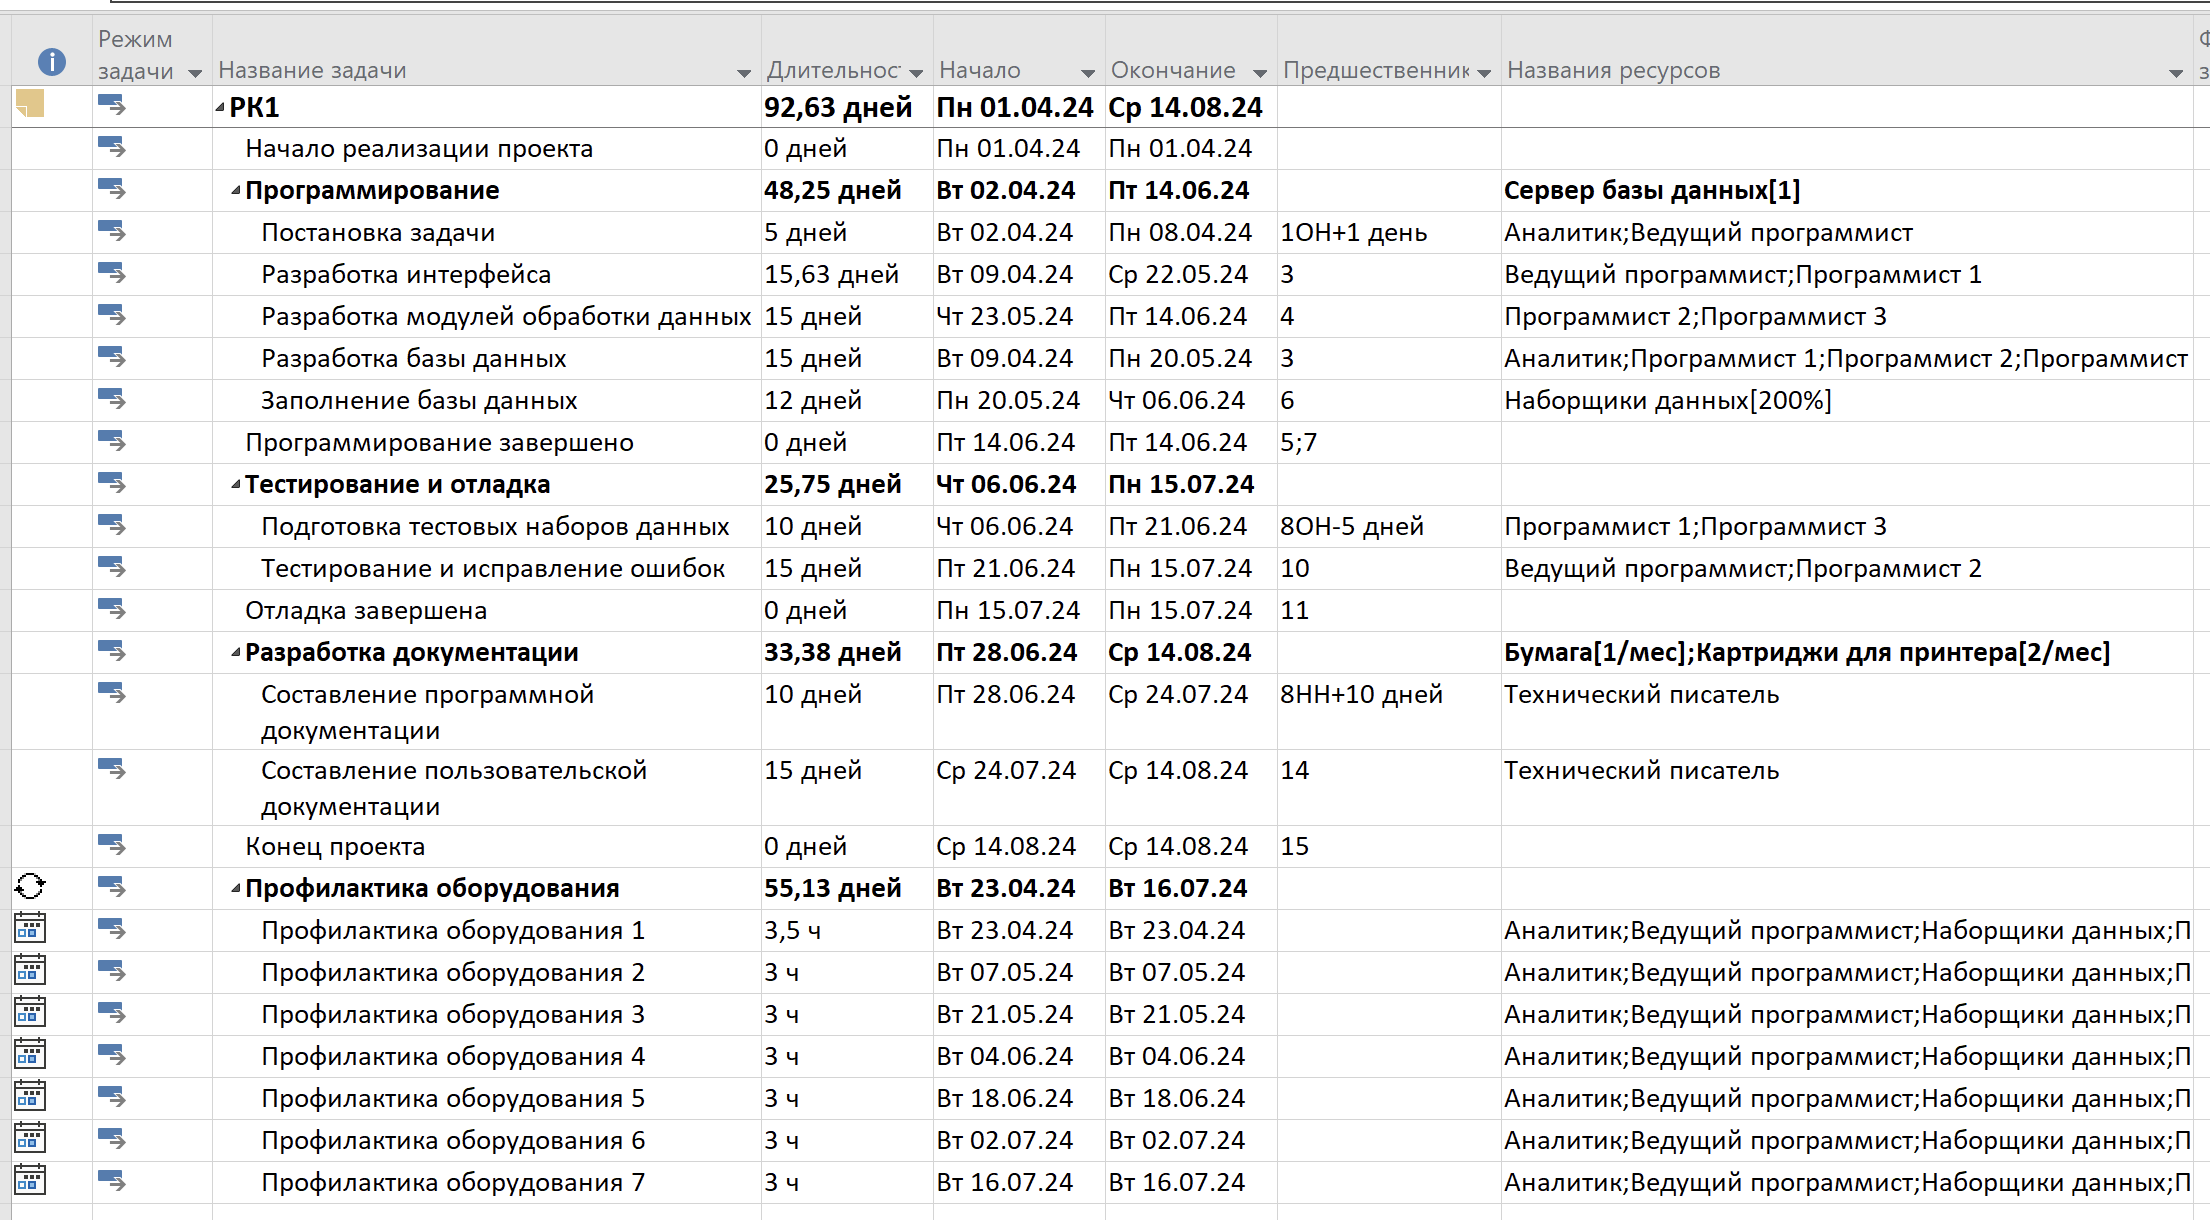
\includegraphics[width=0.75\linewidth]{assets/images/10.5.2-pisaka.png}
	\label{fig:r2}
	\caption{Ухудшаем ситуацию}
\end{figure}
\FloatBarrier

Вывести линию прогресса.

\begin{figure}[ht!]
	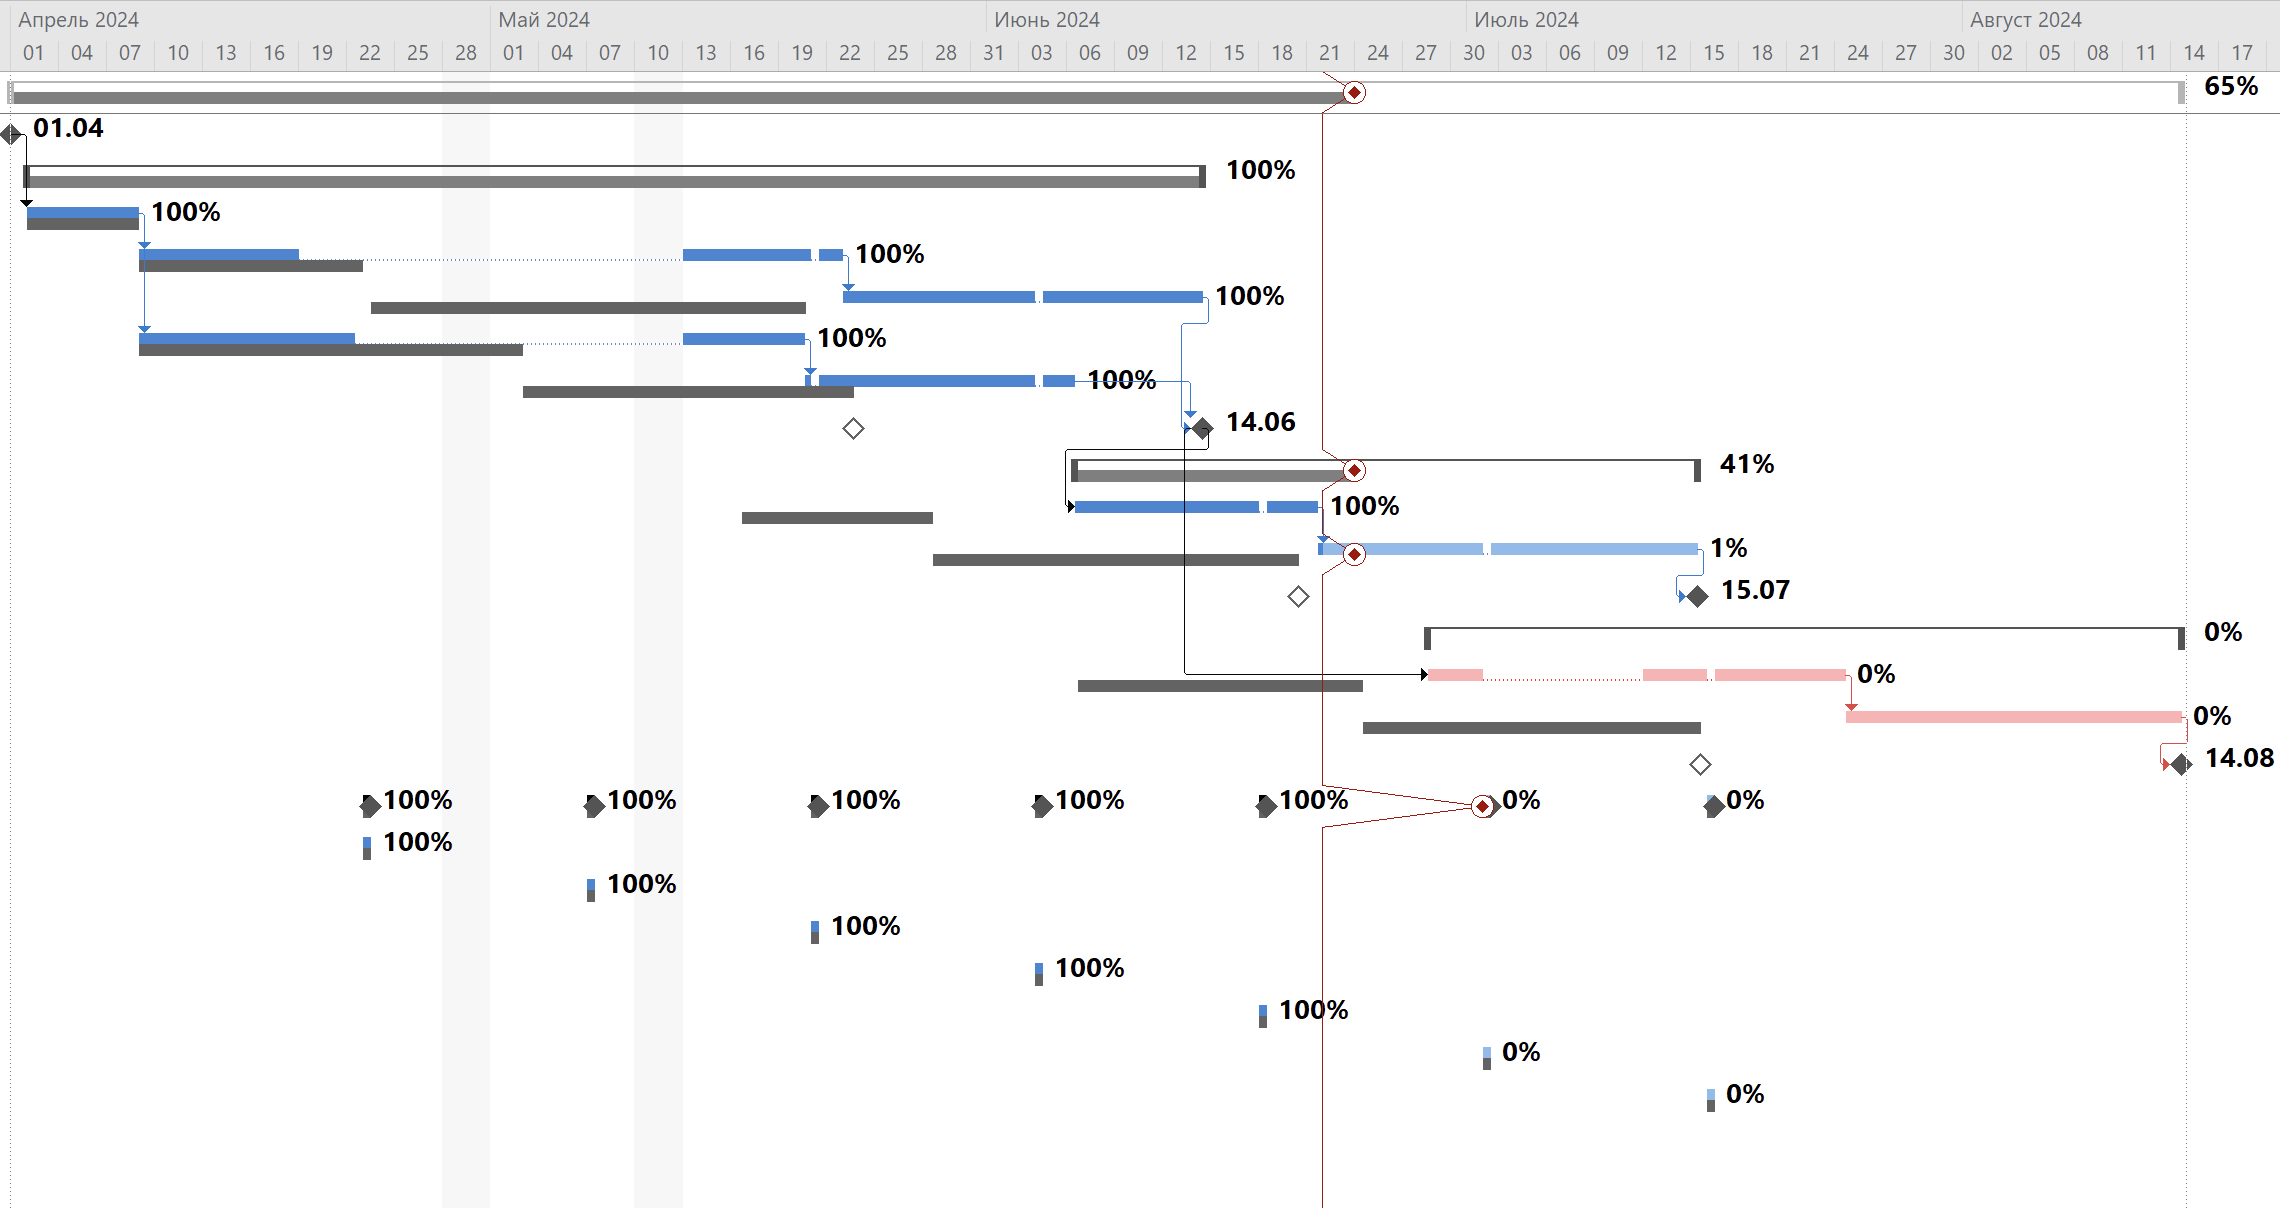
\includegraphics[width=0.75\linewidth]{assets/images/10.5-progress.png}
	\label{fig:r2}
	\caption{Линия прогресса}
\end{figure}
\FloatBarrier


\begin{figure}[ht!]
	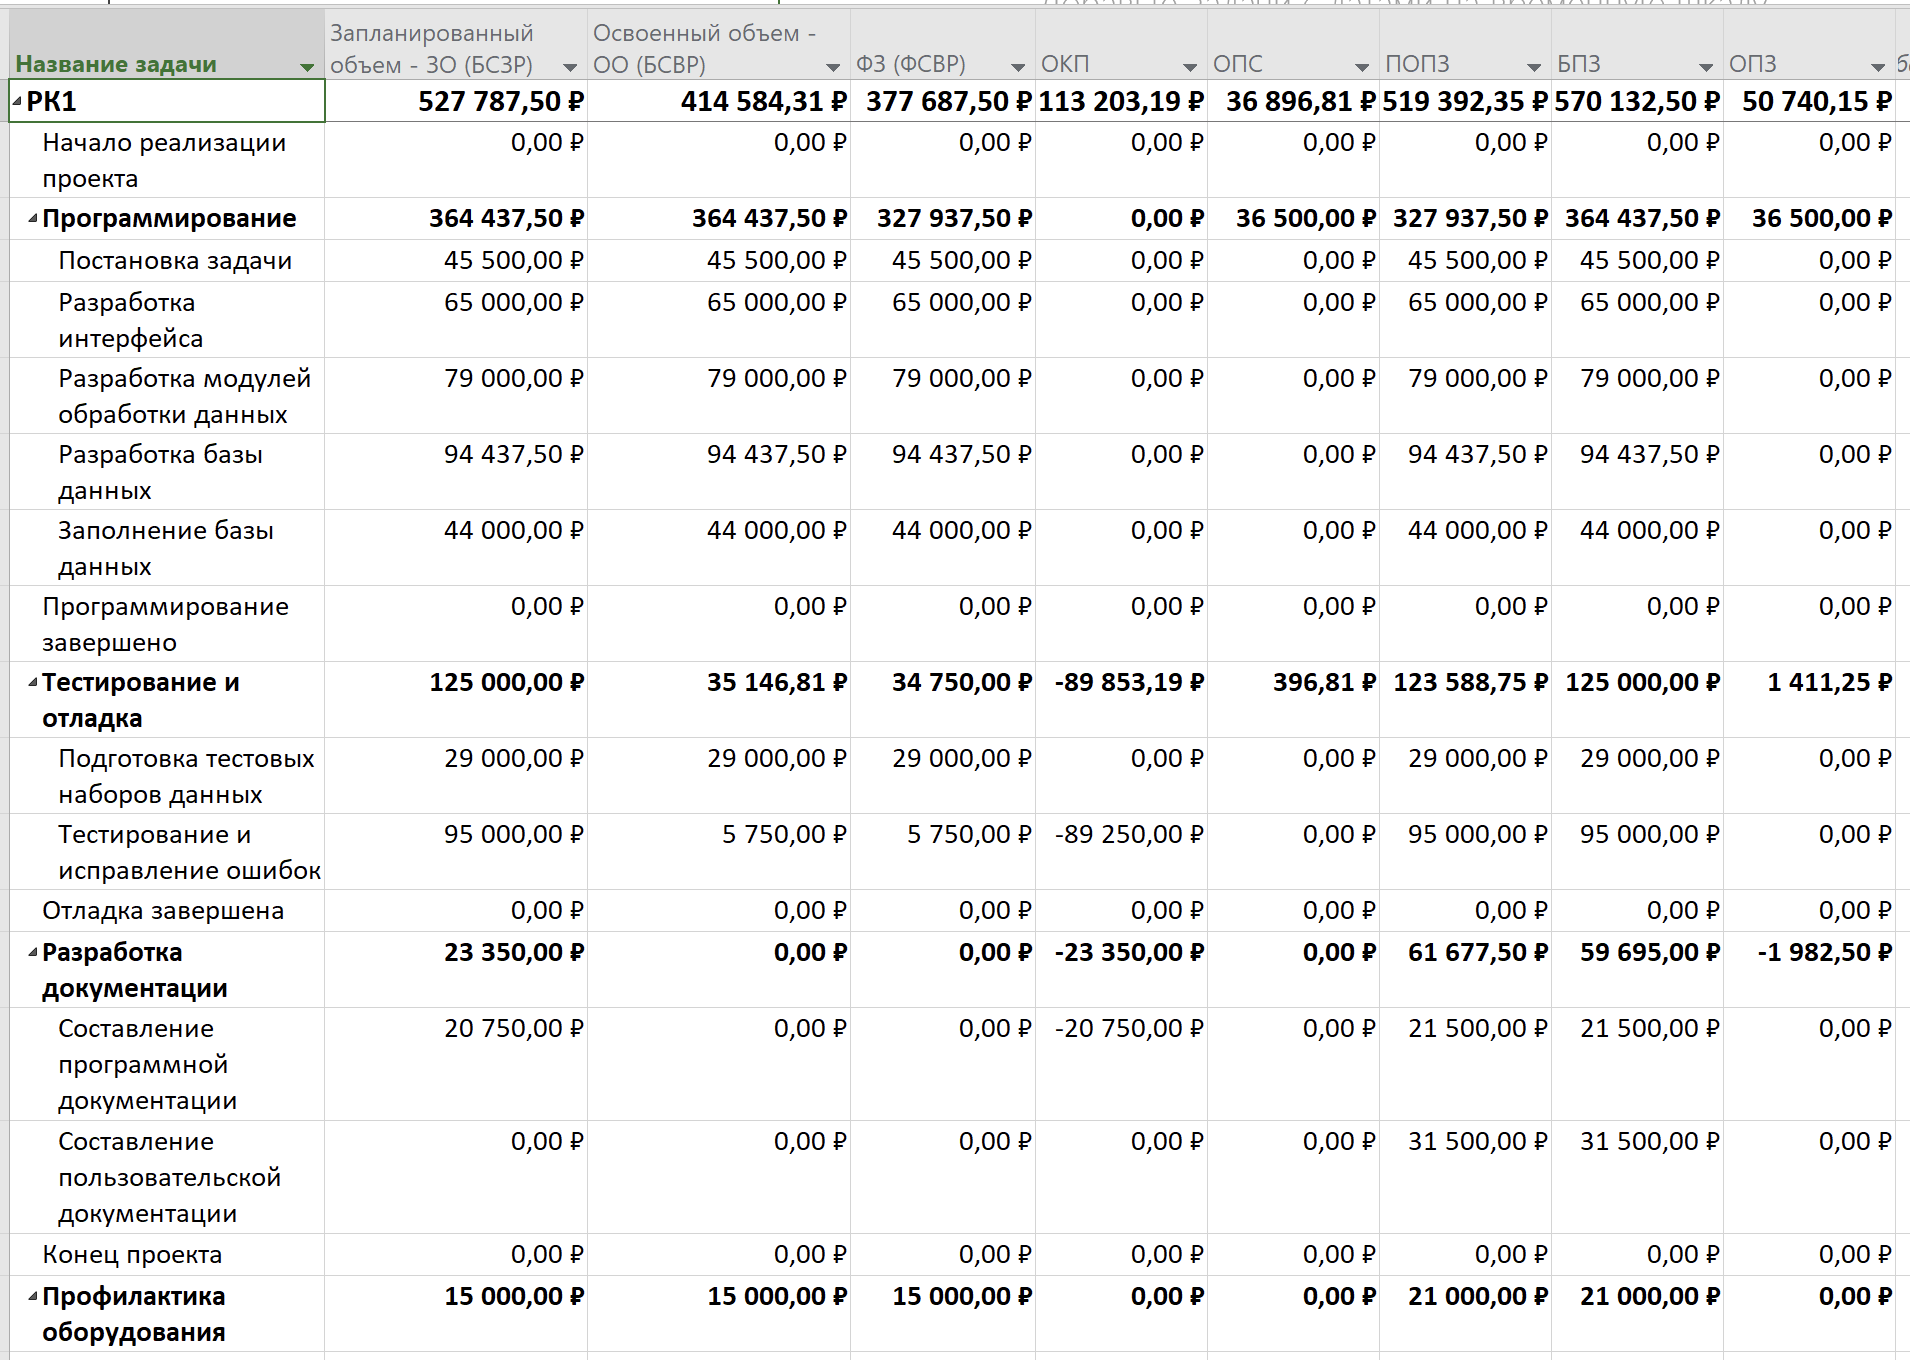
\includegraphics[width=0.75\linewidth]{assets/images/10.6-dengi.png}
	\label{fig:r2}
	\caption{Освоенный объем}
\end{figure}
\FloatBarrier

Основные изменения затронули 11, 13 и 14 задачи.

На 11 задачу повлия то, что программист 1 заболел во время ее выполенения, поэтому задача стала выполняться дольше и ОКП составило -89250.

На 13 задачу повлияло то, что технический писатель заболел во время ее выполнения и ОКП составило -20750.